\documentclass[]{article}
\usepackage{lmodern}
\usepackage{amssymb,amsmath}
\usepackage{ifxetex,ifluatex}
\usepackage{fixltx2e} % provides \textsubscript
\ifnum 0\ifxetex 1\fi\ifluatex 1\fi=0 % if pdftex
  \usepackage[T1]{fontenc}
  \usepackage[utf8]{inputenc}
\else % if luatex or xelatex
  \ifxetex
    \usepackage{mathspec}
  \else
    \usepackage{fontspec}
  \fi
  \defaultfontfeatures{Ligatures=TeX,Scale=MatchLowercase}
\fi
% use upquote if available, for straight quotes in verbatim environments
\IfFileExists{upquote.sty}{\usepackage{upquote}}{}
% use microtype if available
\IfFileExists{microtype.sty}{%
\usepackage{microtype}
\UseMicrotypeSet[protrusion]{basicmath} % disable protrusion for tt fonts
}{}
\usepackage[margin=1in]{geometry}
\usepackage{hyperref}
\hypersetup{unicode=true,
            pdfborder={0 0 0},
            breaklinks=true}
\urlstyle{same}  % don't use monospace font for urls
\usepackage{color}
\usepackage{fancyvrb}
\newcommand{\VerbBar}{|}
\newcommand{\VERB}{\Verb[commandchars=\\\{\}]}
\DefineVerbatimEnvironment{Highlighting}{Verbatim}{commandchars=\\\{\}}
% Add ',fontsize=\small' for more characters per line
\usepackage{framed}
\definecolor{shadecolor}{RGB}{248,248,248}
\newenvironment{Shaded}{\begin{snugshade}}{\end{snugshade}}
\newcommand{\AlertTok}[1]{\textcolor[rgb]{0.94,0.16,0.16}{#1}}
\newcommand{\AnnotationTok}[1]{\textcolor[rgb]{0.56,0.35,0.01}{\textbf{\textit{#1}}}}
\newcommand{\AttributeTok}[1]{\textcolor[rgb]{0.77,0.63,0.00}{#1}}
\newcommand{\BaseNTok}[1]{\textcolor[rgb]{0.00,0.00,0.81}{#1}}
\newcommand{\BuiltInTok}[1]{#1}
\newcommand{\CharTok}[1]{\textcolor[rgb]{0.31,0.60,0.02}{#1}}
\newcommand{\CommentTok}[1]{\textcolor[rgb]{0.56,0.35,0.01}{\textit{#1}}}
\newcommand{\CommentVarTok}[1]{\textcolor[rgb]{0.56,0.35,0.01}{\textbf{\textit{#1}}}}
\newcommand{\ConstantTok}[1]{\textcolor[rgb]{0.00,0.00,0.00}{#1}}
\newcommand{\ControlFlowTok}[1]{\textcolor[rgb]{0.13,0.29,0.53}{\textbf{#1}}}
\newcommand{\DataTypeTok}[1]{\textcolor[rgb]{0.13,0.29,0.53}{#1}}
\newcommand{\DecValTok}[1]{\textcolor[rgb]{0.00,0.00,0.81}{#1}}
\newcommand{\DocumentationTok}[1]{\textcolor[rgb]{0.56,0.35,0.01}{\textbf{\textit{#1}}}}
\newcommand{\ErrorTok}[1]{\textcolor[rgb]{0.64,0.00,0.00}{\textbf{#1}}}
\newcommand{\ExtensionTok}[1]{#1}
\newcommand{\FloatTok}[1]{\textcolor[rgb]{0.00,0.00,0.81}{#1}}
\newcommand{\FunctionTok}[1]{\textcolor[rgb]{0.00,0.00,0.00}{#1}}
\newcommand{\ImportTok}[1]{#1}
\newcommand{\InformationTok}[1]{\textcolor[rgb]{0.56,0.35,0.01}{\textbf{\textit{#1}}}}
\newcommand{\KeywordTok}[1]{\textcolor[rgb]{0.13,0.29,0.53}{\textbf{#1}}}
\newcommand{\NormalTok}[1]{#1}
\newcommand{\OperatorTok}[1]{\textcolor[rgb]{0.81,0.36,0.00}{\textbf{#1}}}
\newcommand{\OtherTok}[1]{\textcolor[rgb]{0.56,0.35,0.01}{#1}}
\newcommand{\PreprocessorTok}[1]{\textcolor[rgb]{0.56,0.35,0.01}{\textit{#1}}}
\newcommand{\RegionMarkerTok}[1]{#1}
\newcommand{\SpecialCharTok}[1]{\textcolor[rgb]{0.00,0.00,0.00}{#1}}
\newcommand{\SpecialStringTok}[1]{\textcolor[rgb]{0.31,0.60,0.02}{#1}}
\newcommand{\StringTok}[1]{\textcolor[rgb]{0.31,0.60,0.02}{#1}}
\newcommand{\VariableTok}[1]{\textcolor[rgb]{0.00,0.00,0.00}{#1}}
\newcommand{\VerbatimStringTok}[1]{\textcolor[rgb]{0.31,0.60,0.02}{#1}}
\newcommand{\WarningTok}[1]{\textcolor[rgb]{0.56,0.35,0.01}{\textbf{\textit{#1}}}}
\usepackage{longtable,booktabs}
\usepackage{graphicx,grffile}
\makeatletter
\def\maxwidth{\ifdim\Gin@nat@width>\linewidth\linewidth\else\Gin@nat@width\fi}
\def\maxheight{\ifdim\Gin@nat@height>\textheight\textheight\else\Gin@nat@height\fi}
\makeatother
% Scale images if necessary, so that they will not overflow the page
% margins by default, and it is still possible to overwrite the defaults
% using explicit options in \includegraphics[width, height, ...]{}
\setkeys{Gin}{width=\maxwidth,height=\maxheight,keepaspectratio}
\IfFileExists{parskip.sty}{%
\usepackage{parskip}
}{% else
\setlength{\parindent}{0pt}
\setlength{\parskip}{6pt plus 2pt minus 1pt}
}
\setlength{\emergencystretch}{3em}  % prevent overfull lines
\providecommand{\tightlist}{%
  \setlength{\itemsep}{0pt}\setlength{\parskip}{0pt}}
\setcounter{secnumdepth}{0}
% Redefines (sub)paragraphs to behave more like sections
\ifx\paragraph\undefined\else
\let\oldparagraph\paragraph
\renewcommand{\paragraph}[1]{\oldparagraph{#1}\mbox{}}
\fi
\ifx\subparagraph\undefined\else
\let\oldsubparagraph\subparagraph
\renewcommand{\subparagraph}[1]{\oldsubparagraph{#1}\mbox{}}
\fi

%%% Use protect on footnotes to avoid problems with footnotes in titles
\let\rmarkdownfootnote\footnote%
\def\footnote{\protect\rmarkdownfootnote}

%%% Change title format to be more compact
\usepackage{titling}

% Create subtitle command for use in maketitle
\providecommand{\subtitle}[1]{
  \posttitle{
    \begin{center}\large#1\end{center}
    }
}

\setlength{\droptitle}{-2em}

  \title{}
    \pretitle{\vspace{\droptitle}}
  \posttitle{}
    \author{}
    \preauthor{}\postauthor{}
    \date{}
    \predate{}\postdate{}
  

\begin{document}

\hypertarget{overview}{%
\section{Overview}\label{overview}}

This document will guide you through some data analysis tasks with a
focus on performing variable selection. For this exercise, we consider a
categorical outcome.

While this is in some sense a stand-alone analysis, I assume that you
have worked through the \emph{Data Analysis} exercise and are familiar
with the dataset and all the things we discovered during the cleaning
process. We'll use the same dataset here but focus on a different
outcome. Other than that, the way to work through the exercise is like
in the \emph{Data Analysis} exercise, namely by writing/completing the
missing code.

\hypertarget{project-setup}{%
\section{Project setup}\label{project-setup}}

We need a variety of different packages, which are loaded here. Install
as needed. If you use others, load them here.

\begin{Shaded}
\begin{Highlighting}[]
\KeywordTok{library}\NormalTok{(}\StringTok{'tidyr'}\NormalTok{)}
\KeywordTok{library}\NormalTok{(}\StringTok{'dplyr'}\NormalTok{)}
\KeywordTok{library}\NormalTok{(}\StringTok{'forcats'}\NormalTok{)}
\KeywordTok{library}\NormalTok{(}\StringTok{'ggplot2'}\NormalTok{)}
\KeywordTok{library}\NormalTok{(}\StringTok{'knitr'}\NormalTok{)}
\KeywordTok{library}\NormalTok{(}\StringTok{'mlr'}\NormalTok{) }\CommentTok{#for model fitting.}
\KeywordTok{library}\NormalTok{(}\StringTok{'parallelMap'}\NormalTok{) }\CommentTok{#for using multiple processors when running models through mlr}
\KeywordTok{library}\NormalTok{(gridExtra)}
\KeywordTok{library}\NormalTok{(visdat)}
\KeywordTok{library}\NormalTok{(pROC)}
\end{Highlighting}
\end{Shaded}

\begin{verbatim}
## Type 'citation("pROC")' for a citation.
\end{verbatim}

\begin{verbatim}
## 
## Attaching package: 'pROC'
\end{verbatim}

\begin{verbatim}
## The following objects are masked from 'package:stats':
## 
##     cov, smooth, var
\end{verbatim}

\hypertarget{data-loading-and-cleaning}{%
\section{Data loading and cleaning}\label{data-loading-and-cleaning}}

We will again use the Norovirus dataset.

\begin{Shaded}
\begin{Highlighting}[]
\CommentTok{#Write code that loads the dataset }
\CommentTok{#You can of course re-use code you wrote in the other file.}
\NormalTok{norodata_raw <-}\StringTok{ }\KeywordTok{read.csv}\NormalTok{(}\StringTok{"./norodata.csv"}\NormalTok{)}

\KeywordTok{glimpse}\NormalTok{(norodata_raw)}
\end{Highlighting}
\end{Shaded}

\begin{verbatim}
## Observations: 1,022
## Variables: 139
## $ id                    <int> 2, 17, 39, 40, 41, 42, 43, 44, 67, 74, 7...
## $ Author                <fct> Akihara, Becker, Boxman, Boxman, Boxman,...
## $ Pub_Year              <int> 2005, 2000, 2009, 2009, 2009, 2009, 2009...
## $ pubmedid              <int> 15841336, 11071673, 19205471, 19205471, ...
## $ EpiCurve              <fct> Y, Y, N, N, N, N, N, N, N, N, Y, Y, Y, Y...
## $ TDComment             <fct> , , , , , , , , , , , , , , , , , , , No...
## $ AHComment             <fct> , , , , , , , , , , , , , , , , , , , , ...
## $ Trans1                <fct> Unspecified, Foodborne, Foodborne, Foodb...
## $ Trans1_O              <int> 0, 0, 0, 0, 0, 0, 0, 0, 0, 0, 0, 0, 0, 0...
## $ Trans2                <fct>   (not applicable), Person to Person,   ...
## $ Trans2_O              <fct> 0, 0, 0, 0, 0, 0, 0, 0, 0, 0, 0, 0, 0, 0...
## $ Trans3                <fct>   (not applicable),   (not applicable), ...
## $ Trans3_O              <fct> 0, 0, 0, 0, 0, 0, 0, 0, 0, 0, 0, 0, 0, 0...
## $ Risk1                 <dbl> 0.00000, 108.00000, 130.00000, 4.00000, ...
## $ Risk2                 <dbl> NA, NA, NA, NA, NA, NA, NA, NA, NA, NA, ...
## $ RiskAll               <dbl> 0.00000, 108.00000, 130.00000, 4.00000, ...
## $ Cases1                <int> 15, 43, 27, 4, 15, 6, 40, 10, 116, 45, 1...
## $ Cases2                <int> NA, 22, NA, NA, NA, NA, NA, NA, NA, NA, ...
## $ CasesAll              <int> 15, 65, 27, 4, 15, 6, 40, 10, 116, 45, 1...
## $ Rate1                 <dbl> NA, 39.814815, 20.769231, 100.000000, 60...
## $ Rate2                 <dbl> NA, NA, NA, NA, NA, NA, NA, NA, NA, NA, ...
## $ RateAll               <dbl> 0.000000, 39.814815, 20.769231, 100.0000...
## $ Hospitalizations      <int> 0, 0, 0, 0, 0, 0, 0, 0, 5, 10, 3, 0, 0, ...
## $ Deaths                <int> 0, 0, 0, 0, 0, 0, 0, 0, 0, 0, 0, 0, 0, 0...
## $ Vehicle_1             <fct> 0, Boxed Lunch, 0, 0, 0, 0, 0, 0, 0, Oys...
## $ Veh1                  <fct> Unspecified, Yes, Unspecified, Unspecifi...
## $ Veh1_D_1              <fct> 0, Turkey Sandwich in boxed lunch, 0, 0,...
## $ Veh2                  <fct> No, Yes, No, No, No, No, No, No, No, No,...
## $ Veh2_D_1              <fct> 0, Football players, 0, 0, 0, 0, 0, 0, 0...
## $ Veh3                  <fct> No, No, No, No, No, No, No, No, No, No, ...
## $ Veh3_D_1              <fct> 0, 0, 0, 0, 0, 0, 0, 0, 0, 0, 0, 0, 0, 0...
## $ PCRSect               <fct> Capsid, Polymerase, Both, Both, Both, Bo...
## $ OBYear                <fct> 1999, 1998, 2006, 2006, 2006, 2006, 2006...
## $ Hemisphere            <fct> Northern, Northern, Northern, Northern, ...
## $ season                <fct> Fall, Fall, Fall, Fall, Fall, Fall, Fall...
## $ MeanI1                <int> 0, 0, 0, 0, 0, 0, 0, 0, 0, 0, 0, 0, 0, 0...
## $ MedianI1              <int> 0, 37, 0, 0, 0, 0, 0, 0, 0, 31, 34, 33, ...
## $ Range_S_I1            <dbl> 0, 0, 0, 0, 0, 0, 0, 0, 0, 2, 0, 6, 0, 0...
## $ Range_L_I1            <dbl> 0, 0, 0, 0, 0, 0, 0, 0, 0, 69, 0, 96, 0,...
## $ MeanD1                <dbl> 0, 0, 0, 0, 0, 0, 0, 0, 0, 0, 0, 0, 24, ...
## $ MedianD1              <dbl> 0, 36, 0, 0, 0, 0, 0, 0, 0, 48, 37, 24, ...
## $ Range_S_D1            <dbl> 0, 0, 0, 0, 0, 0, 0, 0, 0, 10, 0, 5, 4, ...
## $ Range_L_D1            <int> 0, 0, 0, 0, 0, 0, 0, 0, 0, 168, 0, 120, ...
## $ MeanA1                <dbl> NA, NA, NA, NA, NA, NA, NA, NA, NA, NA, ...
## $ MedianA1              <dbl> NA, NA, NA, NA, NA, NA, NA, NA, NA, NA, ...
## $ Range_Y_A1            <fct> 0.75, 0, 0, 0, 0, 0, 0, 0, 0, 0, 0, 0, 0...
## $ Range_O_A1            <dbl> 2, 0, 0, 0, 0, 0, 0, 0, 0, 0, 0, 0, 0, 0...
## $ Action1               <fct> Unspecified, Unspecified, Unspecified, U...
## $ Action2_1             <fct> "0", "0", "0", "0", "0", "0", "0", "0", ...
## $ Secondary             <fct> No, Yes, No, No, No, No, No, No, No, No,...
## $ MeanI2                <int> 0, 0, 0, 0, 0, 0, 0, 0, 0, 0, 0, 0, 0, 0...
## $ MedianI2              <int> 0, 0, 0, 0, 0, 0, 0, 0, 0, 0, 0, 0, 0, 0...
## $ Range_S_I2            <int> 0, 0, 0, 0, 0, 0, 0, 0, 0, 0, 0, 0, 0, 0...
## $ Range_L_I2            <int> 0, 0, 0, 0, 0, 0, 0, 0, 0, 0, 0, 0, 0, 0...
## $ MeanD2                <int> 0, 0, 0, 0, 0, 0, 0, 0, 0, 0, 0, 0, 0, 0...
## $ MedianD2              <int> 0, 0, 0, 0, 0, 0, 0, 0, 0, 0, 0, 0, 0, 0...
## $ Range_S_D2            <int> 0, 0, 0, 0, 0, 0, 0, 0, 0, 0, 0, 0, 0, 0...
## $ Range_L_D2            <int> 0, 0, 0, 0, 0, 0, 0, 0, 0, 0, 0, 0, 0, 0...
## $ Mea.2                 <int> 0, 0, 0, 0, 0, 0, 0, 0, 0, 0, 0, 0, 0, 0...
## $ Media.2               <int> 0, 0, 0, 0, 0, 0, 0, 0, 0, 0, 0, 0, 0, 0...
## $ Range_Y_A2            <int> 0, 0, 0, 0, 0, 0, 0, 0, 0, 0, 0, 0, 0, 0...
## $ Range_O_A2            <int> 0, 0, 0, 0, 0, 0, 0, 0, 0, 0, 0, 0, 0, 0...
## $ Comments_1            <fct> "Outbreak took place during a study on g...
## $ Path1                 <fct> No, No, Unspecified, Unspecified, Unspec...
## $ Path2_1               <fct> 0, 0, 0, 0, 0, 0, 0, 0, 0, 0, 0, 0, 0, 0...
## $ Country               <fct> Japan, USA, Other, Other, Other, Other, ...
## $ Category              <fct> Daycare, Foodservice, Foodservice, Foods...
## $ State                 <fct> "0", "NC, FL", "0", "0", "0", "0", "0", ...
## $ Setting_1             <fct> "Daycare Center", "Boxed lunch, football...
## $ StartMonth            <int> 11, 9, 9, 10, 11, 11, 11, 11, 11, 11, 11...
## $ EndMonth              <int> 12, 9, 0, 0, 0, 0, 0, 0, 11, 11, 11, 11,...
## $ GGA                   <int> 2, 1, 2, 0, 2, 0, 0, 0, 2, 0, 0, 0, 0, 0...
## $ CA                    <int> 4, 0, 4, 0, 4, 0, 0, 0, 4, 0, 0, 0, 0, 0...
## $ SA                    <fct> Lordsdale, Thistle Hall 1/91, GII.4 2006...
## $ new_GGA               <int> 0, 0, 0, 0, 0, 0, 0, 0, 0, 0, 0, 0, 0, 0...
## $ new_CA                <int> 0, 0, 0, 0, 0, 0, 0, 0, 0, 0, 0, 0, 0, 0...
## $ new_SA                <fct> 0, 0, 0, 0, 0, 0, 0, 0, 0, 0, 0, 0, 0, 0...
## $ SA_resolved_from      <fct> , , , , , , , , , , , , , , , , , , , Zh...
## $ GGB                   <int> 0, 0, 0, 0, 0, 0, 0, 0, 0, 0, 0, 0, 0, 0...
## $ CB                    <fct> 0, 0, 0, 0, 0, 0, 0, 0, 0, 0, 0, 0, 0, 0...
## $ SB                    <fct> 0, 0, 0, 0, 0, 0, 0, 0, 0, 0, 0, 0, 0, 0...
## $ new_GGB               <int> 0, 0, 0, 0, 0, 0, 0, 0, 0, 0, 0, 0, 0, 0...
## $ new_CB                <int> 0, 0, 0, 0, 0, 0, 0, 0, 0, 0, 0, 0, 0, 0...
## $ new_SB                <fct> 0, 0, 0, 0, 0, 0, 0, 0, 0, 0, 0, 0, 0, 0...
## $ SB_resolved_from      <fct> , , , , , , , , , , , , , , , , , , http...
## $ GGC                   <int> 0, 0, 0, 0, 0, 0, 0, 0, 0, 0, 0, 0, 0, 0...
## $ CC                    <int> 0, 0, 0, 0, 0, 0, 0, 0, 0, 0, 0, 0, 0, 0...
## $ SC                    <fct> 0, 0, 0, 0, 0, 0, 0, 0, 0, 0, 0, 0, 0, 0...
## $ new_ggc               <int> 0, 0, 0, 0, 0, 0, 0, 0, 0, 0, 0, 0, 0, 0...
## $ new_cc                <int> 0, 0, 0, 0, 0, 0, 0, 0, 0, 0, 0, 0, 0, 0...
## $ new_sc                <fct> 0, 0, 0, 0, 0, 0, 0, 0, 0, 0, 0, 0, 0, 0...
## $ SC_resolved_from      <fct> , , , , , , , , , , , , , , , , , , , , ...
## $ GGD                   <int> 0, 0, 0, 0, 0, 0, 0, 0, 0, 0, 0, 0, 0, 0...
## $ CD                    <fct> 0, 0, 0, 0, 0, 0, 0, 0, 0, 0, 0, 0, 0, 0...
## $ SD                    <fct> 0, 0, 0, 0, 0, 0, 0, 0, 0, 0, 0, 0, 0, 0...
## $ new_ggd               <int> 0, 0, 0, 0, 0, 0, 0, 0, 0, 0, 0, 0, 0, 0...
## $ new_cd                <int> 0, 0, 0, 0, 0, 0, 0, 0, 0, 0, 0, 0, 0, 0...
## $ new_sd                <int> 0, 0, 0, 0, 0, 0, 0, 0, 0, 0, 0, 0, 0, 0...
## $ SD_resolved_from      <lgl> NA, NA, NA, NA, NA, NA, NA, NA, NA, NA, ...
## $ StrainOther           <fct> "0", "0", "0", "0", "0", "0", "0", "0", ...
## $ strainother_rc        <fct> 0, 0, 0, 0, 0, 0, 0, 0, 0, 0, 0, 0, 0, 0...
## $ gge                   <fct> 0, 0, 0, 0, 0, 0, 0, 0, 2, 0, 0, 0, 0, 0...
## $ ce                    <int> 0, 0, 0, 0, 0, 0, 0, 0, 4, 0, 0, 0, 0, 0...
## $ se                    <fct> 0, 0, 0, 0, 0, 0, 0, 0, GII.4a 2004, 0, ...
## $ SE_resolved_from      <fct> , , , , , , , , abstraction of StrainOth...
## $ ggf                   <int> 0, 0, 0, 0, 0, 0, 0, 0, 0, 0, 0, 0, 0, 0...
## $ cf                    <int> 0, 0, 0, 0, 0, 0, 0, 0, 0, 0, 0, 0, 0, 0...
## $ sf                    <fct> 0, 0, 0, 0, 0, 0, 0, 0, 0, 0, 0, 0, 0, 0...
## $ ggg                   <int> 0, 0, 0, 0, 0, 0, 0, 0, 0, 0, 0, 0, 0, 0...
## $ cg                    <int> 0, 0, 0, 0, 0, 0, 0, 0, 0, 0, 0, 0, 0, 0...
## $ sg                    <fct> 0, 0, 0, 0, 0, 0, 0, 0, 0, 0, 0, 0, 0, 0...
## $ ggh                   <int> 0, 0, 0, 0, 0, 0, 0, 0, 0, 0, 0, 0, 0, 0...
## $ ch                    <int> 0, 0, 0, 0, 0, 0, 0, 0, 0, 0, 0, 0, 0, 0...
## $ sh                    <fct> 0, 0, 0, 0, 0, 0, 0, 0, 0, 0, 0, 0, 0, 0...
## $ ggi                   <int> 0, 0, 0, 0, 0, 0, 0, 0, 0, 0, 0, 0, 0, 0...
## $ ci                    <int> 0, 0, 0, 0, 0, 0, 0, 0, 0, 0, 0, 0, 0, 0...
## $ si                    <fct> 0, 0, 0, 0, 0, 0, 0, 0, 0, 0, 0, 0, 0, 0...
## $ ggj                   <int> 0, 0, 0, 0, 0, 0, 0, 0, 0, 0, 0, 0, 0, 0...
## $ cj                    <int> 0, 0, 0, 0, 0, 0, 0, 0, 0, 0, 0, 0, 0, 0...
## $ sj                    <fct> 0, 0, 0, 0, 0, 0, 0, 0, 0, 0, 0, 0, 0, 0...
## $ Country2              <fct> "0", "0", "The Netherlands", "The Nether...
## $ Veh1_D_2              <fct> "0", "Boxed Lunch", "0", "0", "0", "0", ...
## $ Veh2_D_2              <fct> 0, 0, 0, 0, 0, 0, 0, 0, 0, 0, 0, 0, 0, 0...
## $ Veh3_D_2              <fct> 0, 0, 0, 0, 0, 0, 0, 0, 0, 0, 0, 0, 0, 0...
## $ Action2_2             <fct> "0", "0", "0", "0", "0", "0", "0", "0", ...
## $ Comments_2            <fct> "Limited data", "0", "Outbreak 19 of 26 ...
## $ Path2_2               <fct> 0, 0, 0, 0, 0, 0, 0, 0, 0, 0, 0, 0, 0, 0...
## $ Setting_2             <fct> 0, 0, Buffet, Restaurant, Buffet, take o...
## $ category1             <fct> School/Daycare, Foodservice, Foodservice...
## $ strainothergg2c4      <int> 0, 0, 0, 0, 0, 0, 0, 0, 0, 0, 0, 0, 0, 0...
## $ gg2c4                 <fct> Yes, , Yes, , Yes, , , , Yes, , , , , , ...
## $ Vomit                 <int> 1, 1, 1, 1, 1, 1, 1, 1, 1, 1, 1, 1, 1, 1...
## $ IncInd                <int> 0, 0, 0, 0, 0, 0, 0, 0, 0, 0, 0, 0, 0, 0...
## $ SymInd                <int> 0, 0, 0, 0, 0, 0, 0, 0, 0, 0, 0, 0, 0, 0...
## $ PooledLat             <dbl> 0, 37, 0, 0, 0, 0, 0, 0, 0, 31, 34, 33, ...
## $ PooledSym             <int> 0, 36, 0, 0, 0, 0, 0, 0, 0, 48, 37, 24, ...
## $ PooledAge             <dbl> 0, 0, 0, 0, 0, 0, 0, 0, 0, 0, 0, 0, 0, 0...
## $ IndividualLatent      <lgl> NA, NA, NA, NA, NA, NA, NA, NA, NA, NA, ...
## $ IndividualSymptomatic <fct> , , , , , , , , , , , , , , , , , , , , ...
\end{verbatim}

\hypertarget{looking-at-the-outcome}{%
\section{Looking at the outcome}\label{looking-at-the-outcome}}

For this analysis, our main outcome of interest is if an outbreak was
caused by the G2.4 strain of norovirus or not, and how other factors
might be correlated with that strain.

\begin{Shaded}
\begin{Highlighting}[]
\CommentTok{#write code to take a look at the outcome variable (gg2c4)}
\KeywordTok{table}\NormalTok{(norodata_raw}\OperatorTok{$}\NormalTok{gg2c4)}
\end{Highlighting}
\end{Shaded}

\begin{verbatim}
## 
##     Yes 
## 716 306
\end{verbatim}

\begin{Shaded}
\begin{Highlighting}[]
\KeywordTok{print}\NormalTok{(norodata_raw}\OperatorTok{$}\NormalTok{gg2c4)}
\end{Highlighting}
\end{Shaded}

\begin{verbatim}
##    [1] Yes     Yes     Yes             Yes                                
##   [18]     Yes     Yes Yes Yes Yes Yes Yes Yes Yes Yes Yes Yes Yes Yes    
##   [35] Yes Yes Yes         Yes                                         Yes
##   [52] Yes             Yes         Yes                     Yes            
##   [69] Yes         Yes                         Yes Yes Yes Yes Yes        
##   [86]         Yes                     Yes Yes Yes     Yes                
##  [103]         Yes Yes                                 Yes Yes         Yes
##  [120] Yes Yes     Yes Yes Yes Yes Yes Yes Yes Yes Yes Yes                
##  [137]                         Yes                 Yes Yes                
##  [154]                                 Yes Yes         Yes                
##  [171]     Yes Yes Yes Yes                                 Yes            
##  [188] Yes Yes Yes Yes     Yes Yes             Yes Yes Yes     Yes Yes    
##  [205]                                                                    
##  [222]                                     Yes         Yes                
##  [239]                                 Yes                                
##  [256]                         Yes     Yes                                
##  [273]     Yes                     Yes             Yes                    
##  [290] Yes                                                             Yes
##  [307]                         Yes     Yes Yes                            
##  [324]                                             Yes Yes                
##  [341]     Yes Yes         Yes                         Yes Yes Yes Yes    
##  [358]                 Yes Yes                             Yes     Yes    
##  [375] Yes     Yes                                                        
##  [392]     Yes Yes Yes Yes             Yes Yes             Yes            
##  [409]         Yes             Yes             Yes             Yes Yes Yes
##  [426]                     Yes         Yes         Yes Yes     Yes        
##  [443]                                         Yes                        
##  [460] Yes                                                                
##  [477]                 Yes                 Yes Yes Yes Yes Yes Yes        
##  [494]                                             Yes                 Yes
##  [511]                     Yes     Yes             Yes                    
##  [528]                                         Yes Yes     Yes Yes Yes Yes
##  [545] Yes Yes Yes Yes                 Yes     Yes Yes Yes             Yes
##  [562] Yes Yes                                                            
##  [579]     Yes                                     Yes             Yes    
##  [596]                                                                    
##  [613]                                                                    
##  [630]                                                         Yes Yes    
##  [647]             Yes     Yes         Yes Yes Yes Yes     Yes Yes        
##  [664] Yes Yes                     Yes                                 Yes
##  [681]         Yes         Yes         Yes Yes             Yes            
##  [698]                 Yes                     Yes     Yes     Yes Yes    
##  [715]         Yes                         Yes             Yes            
##  [732] Yes Yes Yes         Yes     Yes Yes     Yes Yes Yes Yes Yes Yes Yes
##  [749] Yes Yes Yes     Yes Yes                 Yes Yes Yes     Yes Yes Yes
##  [766]     Yes     Yes Yes Yes     Yes         Yes     Yes                
##  [783]                                 Yes         Yes Yes Yes            
##  [800]                                     Yes                            
##  [817]                                             Yes         Yes Yes    
##  [834]             Yes     Yes             Yes Yes Yes     Yes     Yes Yes
##  [851]     Yes Yes     Yes Yes Yes Yes Yes Yes Yes Yes Yes Yes            
##  [868]                             Yes     Yes Yes Yes     Yes     Yes Yes
##  [885] Yes Yes                                                         Yes
##  [902] Yes Yes Yes                                     Yes Yes Yes Yes Yes
##  [919]     Yes Yes     Yes Yes Yes Yes Yes Yes Yes     Yes     Yes Yes    
##  [936] Yes Yes         Yes                                                
##  [953]                                         Yes         Yes            
##  [970]                             Yes     Yes Yes Yes Yes Yes Yes Yes Yes
##  [987] Yes Yes                                 Yes Yes Yes Yes Yes Yes    
## [1004] Yes Yes Yes Yes Yes                             Yes     Yes     Yes
## [1021] Yes Yes
## Levels:  Yes
\end{verbatim}

Overall, it looks ok, a decent amout in each category (i.e.~no
unbalanced data). However, we see an odd coding, there are only 2 types
of entries, either ``Yes'' or "``, i.e.~an empty space. The codebook
tells us that this is how things were coded, if it was G2.4 it got
a''Yes``, if it wasn't it did get an empty space instead of a''No``.
That's somewhat strange and while the analysis should work, it is better
to re-code the empty slots with''No".

\begin{Shaded}
\begin{Highlighting}[]
\CommentTok{#write code to change the empty values in gg2c4 to "No"}

\NormalTok{norodata_raw}\OperatorTok{$}\NormalTok{gg2c4[}\KeywordTok{which}\NormalTok{(norodata_raw}\OperatorTok{$}\NormalTok{gg2c4}\OperatorTok{==}\StringTok{""}\NormalTok{)] <-}\StringTok{ "No"} 
\end{Highlighting}
\end{Shaded}

\begin{verbatim}
## Warning in `[<-.factor`(`*tmp*`, which(norodata_raw$gg2c4 == ""), value =
## structure(c(2L, : invalid factor level, NA generated
\end{verbatim}

\begin{Shaded}
\begin{Highlighting}[]
\KeywordTok{glimpse}\NormalTok{(norodata_raw}\OperatorTok{$}\NormalTok{gg2c4) }\CommentTok{#this makes No as NA so we'll try and fix it}
\end{Highlighting}
\end{Shaded}

\begin{verbatim}
##  Factor w/ 2 levels "","Yes": 2 NA 2 NA 2 NA NA NA 2 NA ...
\end{verbatim}

\begin{Shaded}
\begin{Highlighting}[]
\NormalTok{norodata_raw}\OperatorTok{$}\NormalTok{gg2c4 <-}\StringTok{ }\KeywordTok{as.character}\NormalTok{(norodata_raw}\OperatorTok{$}\NormalTok{gg2c4)}

\NormalTok{norodata_raw}\OperatorTok{$}\NormalTok{gg2c4[}\KeywordTok{is.na}\NormalTok{(norodata_raw}\OperatorTok{$}\NormalTok{gg2c4)] <-}\StringTok{ "No"}

\KeywordTok{glimpse}\NormalTok{(norodata_raw}\OperatorTok{$}\NormalTok{gg2c4)}
\end{Highlighting}
\end{Shaded}

\begin{verbatim}
##  chr [1:1022] "Yes" "No" "Yes" "No" "Yes" "No" "No" "No" "Yes" "No" ...
\end{verbatim}

\begin{Shaded}
\begin{Highlighting}[]
\CommentTok{#lovely}
\end{Highlighting}
\end{Shaded}

\hypertarget{selecting-predictors}{%
\section{Selecting predictors}\label{selecting-predictors}}

We will pick similar variables as previously, with some adjustments
based on what we learned before. Keep the following variables:
\texttt{Action1,\ CasesAll,\ Country,\ Deaths,\ GG2C4,\ Hemisphere,\ Hospitalizations,\ \ MeanD1,\ MeanI1,\ MedianD1,\ MedianI1,\ OBYear,\ Path1,\ RiskAll,\ Season,\ Setting,\ Trans1,\ Vomit.}

\begin{Shaded}
\begin{Highlighting}[]
\NormalTok{norodata_rawv <-}\StringTok{ }\NormalTok{norodata_raw }\OperatorTok\StringTok{ }\NormalTok{dplyr}\OperatorTok{::}\KeywordTok{select}\NormalTok{(Action1, CasesAll, Country, Deaths, gg2c4, Hemisphere, Hospitalizations,  MeanD1, MeanI1, MedianD1, MedianI1, OBYear, Path1, RiskAll, season, Setting_}\DecValTok{1}\NormalTok{, Trans1, Vomit)}
\KeywordTok{dim}\NormalTok{(norodata_rawv)}
\end{Highlighting}
\end{Shaded}

\begin{verbatim}
## [1] 1022   18
\end{verbatim}

\hypertarget{cleaning-predictors}{%
\section{Cleaning predictors}\label{cleaning-predictors}}

We'll likely have to perform similar cleaning steps as before. A
difference is that earlier we had to drop about half of the observations
because no outcome was available. Here, we have outcome for every
outbreak. Thus, there is more data to clean, which - as we will see -
introduces a few issues we didn't have before, since we dropped the
troublesome observations early in the process.

Let's first check for missing values.

\begin{Shaded}
\begin{Highlighting}[]
\CommentTok{# write code that looks at missing values}
\KeywordTok{vis_miss}\NormalTok{(norodata_rawv)}
\end{Highlighting}
\end{Shaded}

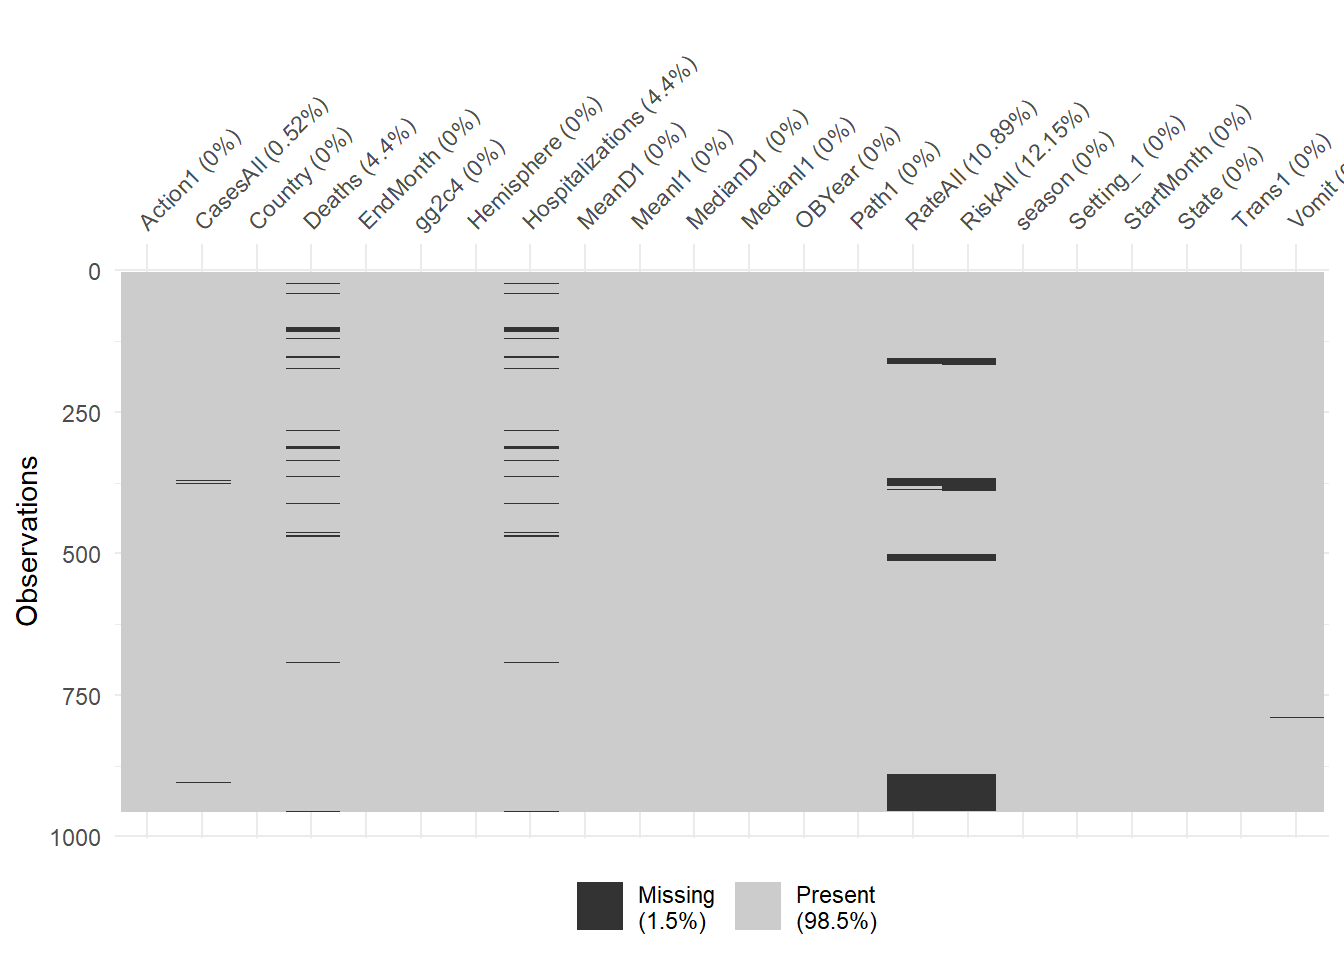
\includegraphics{Variable_Selection_files/figure-latex/check-reduced-data-1.pdf}

Looks like we have again some missing in \texttt{Hospitalization} and
\texttt{Deaths}, and some more in \texttt{RiskAll}. Since the missing is
not excessive, and to make our life easier, we'll drop them for now.
Note however the `blocks' of missing values for RiskAll. Given that
these outbreaks should be entered fairly randomly into the spreadsheet,
it is strange to see the NA show up in such blocks. For a real data
analysis, it would be worth looking closer and checking why there is a
clustering like that.

\begin{Shaded}
\begin{Highlighting}[]
\CommentTok{# write code to remove any observations with NA}
\NormalTok{removena_noro <-}\StringTok{ }\KeywordTok{na.omit}\NormalTok{(norodata_rawv)}
\KeywordTok{vis_miss}\NormalTok{(removena_noro)}
\end{Highlighting}
\end{Shaded}

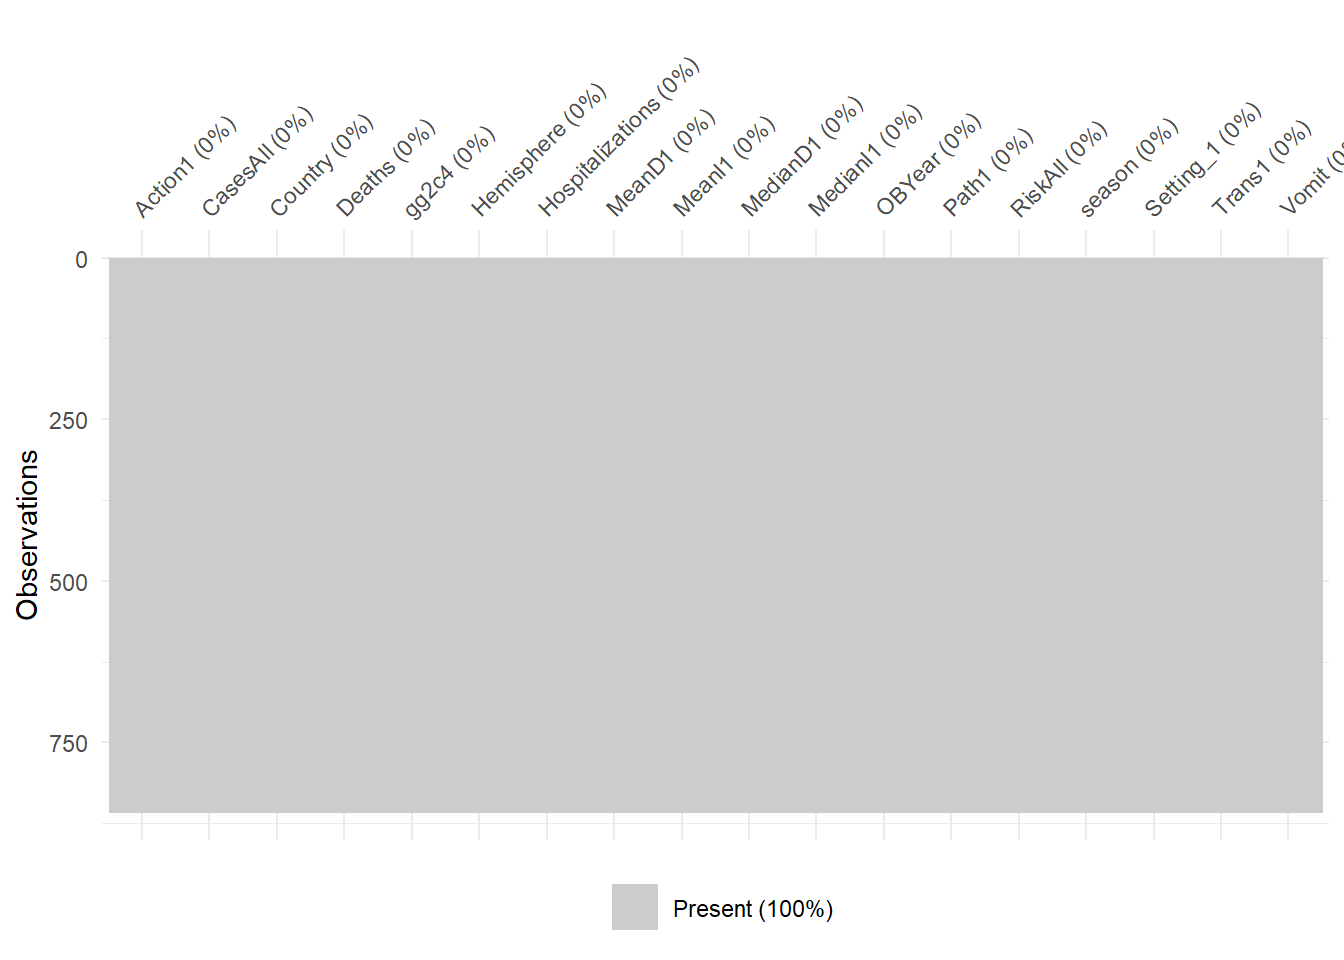
\includegraphics{Variable_Selection_files/figure-latex/further-reduce-data-1.pdf}

Let's make sure everything has the right format
(numeric/integer/factor). Adjust/recode variables as needed. You will
likely find that as you convert \texttt{OBYear} to numeric, something
doesn't quite work. Take a look. Fix by removing the observation with
the troublesome entry, then convert to numeric. Finally, remove the
observations that have 0 as OByear - there are more than 1 now.

\begin{Shaded}
\begin{Highlighting}[]
\CommentTok{#write code that cleans OBYear, convert it to numeric. Remove observations with OBYear = 0. }
\KeywordTok{unique}\NormalTok{(removena_noro}\OperatorTok{$}\NormalTok{OBYear)}
\end{Highlighting}
\end{Shaded}

\begin{verbatim}
##  [1] 1999 1998 2006 2004 1993 2002 2005 2003 1994 2008 2000 2001 1997 1995
## [15] 1996 2007 2009 1990 0    1983 2010 1992
## 23 Levels: 0 1983 1990 1992 1993 1994 1995 1996 1997 1998 1999 ... 2010
\end{verbatim}

\begin{Shaded}
\begin{Highlighting}[]
\KeywordTok{print}\NormalTok{(removena_noro}\OperatorTok{$}\NormalTok{OBYear }\OperatorTok{==}\StringTok{ "1983"}\NormalTok{)}
\end{Highlighting}
\end{Shaded}

\begin{verbatim}
##   [1] FALSE FALSE FALSE FALSE FALSE FALSE FALSE FALSE FALSE FALSE FALSE
##  [12] FALSE FALSE FALSE FALSE FALSE FALSE FALSE FALSE FALSE FALSE FALSE
##  [23] FALSE FALSE FALSE FALSE FALSE FALSE FALSE FALSE FALSE FALSE FALSE
##  [34] FALSE FALSE FALSE FALSE FALSE FALSE FALSE FALSE FALSE FALSE FALSE
##  [45] FALSE FALSE FALSE FALSE FALSE FALSE FALSE FALSE FALSE FALSE FALSE
##  [56] FALSE FALSE FALSE FALSE FALSE FALSE FALSE FALSE FALSE FALSE FALSE
##  [67] FALSE FALSE FALSE FALSE FALSE FALSE FALSE FALSE FALSE FALSE FALSE
##  [78] FALSE FALSE FALSE FALSE FALSE FALSE FALSE FALSE FALSE FALSE FALSE
##  [89] FALSE FALSE FALSE FALSE FALSE FALSE FALSE FALSE FALSE FALSE FALSE
## [100] FALSE FALSE FALSE FALSE FALSE FALSE FALSE FALSE FALSE FALSE FALSE
## [111] FALSE FALSE FALSE FALSE FALSE FALSE FALSE FALSE FALSE FALSE FALSE
## [122] FALSE FALSE FALSE FALSE FALSE FALSE FALSE FALSE FALSE FALSE FALSE
## [133] FALSE FALSE FALSE FALSE FALSE FALSE FALSE FALSE FALSE FALSE FALSE
## [144] FALSE FALSE FALSE FALSE FALSE FALSE FALSE FALSE FALSE FALSE FALSE
## [155] FALSE FALSE FALSE FALSE FALSE FALSE FALSE FALSE FALSE FALSE FALSE
## [166] FALSE FALSE FALSE FALSE FALSE FALSE FALSE FALSE FALSE FALSE FALSE
## [177] FALSE FALSE FALSE FALSE FALSE FALSE FALSE FALSE FALSE FALSE FALSE
## [188] FALSE FALSE FALSE FALSE FALSE FALSE FALSE FALSE FALSE FALSE FALSE
## [199] FALSE FALSE FALSE FALSE FALSE FALSE FALSE FALSE FALSE FALSE FALSE
## [210] FALSE FALSE FALSE FALSE FALSE FALSE FALSE FALSE FALSE FALSE FALSE
## [221] FALSE FALSE FALSE FALSE FALSE FALSE FALSE FALSE FALSE FALSE FALSE
## [232] FALSE FALSE FALSE FALSE FALSE FALSE FALSE FALSE FALSE FALSE FALSE
## [243] FALSE FALSE FALSE FALSE FALSE FALSE FALSE FALSE FALSE FALSE FALSE
## [254] FALSE FALSE FALSE FALSE FALSE FALSE FALSE FALSE FALSE FALSE FALSE
## [265] FALSE FALSE FALSE FALSE FALSE FALSE FALSE FALSE FALSE FALSE FALSE
## [276] FALSE FALSE FALSE FALSE FALSE FALSE FALSE FALSE FALSE FALSE FALSE
## [287] FALSE FALSE FALSE FALSE FALSE FALSE FALSE FALSE FALSE FALSE FALSE
## [298] FALSE FALSE FALSE FALSE FALSE FALSE FALSE FALSE FALSE FALSE FALSE
## [309] FALSE FALSE FALSE FALSE FALSE FALSE FALSE FALSE FALSE FALSE FALSE
## [320] FALSE FALSE FALSE FALSE FALSE FALSE FALSE FALSE FALSE FALSE FALSE
## [331] FALSE FALSE FALSE FALSE FALSE FALSE FALSE FALSE FALSE FALSE FALSE
## [342] FALSE FALSE FALSE FALSE FALSE FALSE FALSE FALSE FALSE FALSE FALSE
## [353] FALSE FALSE FALSE FALSE FALSE FALSE FALSE FALSE FALSE FALSE FALSE
## [364] FALSE FALSE FALSE FALSE FALSE FALSE FALSE FALSE FALSE FALSE FALSE
## [375] FALSE FALSE FALSE FALSE FALSE FALSE FALSE FALSE FALSE FALSE FALSE
## [386] FALSE FALSE FALSE FALSE FALSE FALSE FALSE FALSE FALSE FALSE FALSE
## [397] FALSE FALSE FALSE FALSE FALSE FALSE FALSE FALSE FALSE FALSE FALSE
## [408]  TRUE FALSE FALSE FALSE FALSE FALSE FALSE FALSE FALSE FALSE FALSE
## [419] FALSE FALSE FALSE FALSE FALSE FALSE FALSE FALSE FALSE FALSE FALSE
## [430] FALSE FALSE FALSE FALSE FALSE FALSE FALSE FALSE FALSE FALSE FALSE
## [441] FALSE FALSE FALSE FALSE FALSE FALSE FALSE FALSE FALSE FALSE FALSE
## [452] FALSE FALSE FALSE FALSE FALSE FALSE FALSE FALSE FALSE FALSE FALSE
## [463] FALSE FALSE FALSE FALSE FALSE FALSE FALSE FALSE FALSE FALSE FALSE
## [474] FALSE FALSE FALSE FALSE FALSE FALSE FALSE FALSE FALSE FALSE FALSE
## [485] FALSE FALSE FALSE FALSE FALSE FALSE FALSE FALSE FALSE FALSE FALSE
## [496] FALSE FALSE FALSE FALSE FALSE FALSE FALSE FALSE FALSE FALSE FALSE
## [507] FALSE FALSE FALSE FALSE FALSE FALSE FALSE FALSE FALSE FALSE FALSE
## [518] FALSE FALSE FALSE FALSE FALSE FALSE FALSE FALSE FALSE FALSE FALSE
## [529] FALSE FALSE FALSE FALSE FALSE FALSE FALSE FALSE FALSE FALSE FALSE
## [540] FALSE FALSE FALSE FALSE FALSE FALSE FALSE FALSE FALSE FALSE FALSE
## [551] FALSE FALSE FALSE FALSE FALSE FALSE FALSE FALSE FALSE FALSE FALSE
## [562] FALSE FALSE FALSE FALSE FALSE FALSE FALSE FALSE FALSE FALSE FALSE
## [573] FALSE FALSE FALSE FALSE FALSE FALSE FALSE FALSE FALSE FALSE FALSE
## [584] FALSE FALSE FALSE FALSE FALSE FALSE FALSE FALSE FALSE FALSE FALSE
## [595] FALSE FALSE FALSE FALSE FALSE FALSE FALSE FALSE FALSE FALSE FALSE
## [606] FALSE FALSE FALSE FALSE FALSE FALSE FALSE FALSE FALSE FALSE FALSE
## [617] FALSE FALSE FALSE FALSE FALSE FALSE FALSE FALSE FALSE FALSE FALSE
## [628] FALSE FALSE FALSE FALSE FALSE FALSE FALSE FALSE FALSE FALSE FALSE
## [639] FALSE FALSE FALSE FALSE FALSE FALSE FALSE FALSE FALSE FALSE FALSE
## [650] FALSE FALSE FALSE FALSE FALSE FALSE FALSE FALSE FALSE FALSE FALSE
## [661] FALSE FALSE FALSE FALSE FALSE FALSE FALSE FALSE FALSE FALSE FALSE
## [672] FALSE FALSE FALSE FALSE FALSE FALSE FALSE FALSE FALSE FALSE FALSE
## [683] FALSE FALSE FALSE FALSE FALSE FALSE FALSE FALSE FALSE FALSE FALSE
## [694] FALSE FALSE FALSE FALSE FALSE FALSE FALSE FALSE FALSE FALSE FALSE
## [705] FALSE FALSE FALSE FALSE FALSE FALSE FALSE FALSE FALSE FALSE FALSE
## [716] FALSE FALSE FALSE FALSE FALSE FALSE FALSE FALSE FALSE FALSE FALSE
## [727] FALSE FALSE FALSE FALSE FALSE FALSE FALSE FALSE FALSE FALSE FALSE
## [738] FALSE FALSE FALSE FALSE FALSE FALSE FALSE FALSE FALSE FALSE FALSE
## [749] FALSE FALSE FALSE FALSE FALSE FALSE FALSE FALSE FALSE FALSE FALSE
## [760] FALSE FALSE FALSE FALSE FALSE FALSE FALSE FALSE FALSE FALSE FALSE
## [771] FALSE FALSE FALSE FALSE FALSE FALSE FALSE FALSE FALSE FALSE FALSE
## [782] FALSE FALSE FALSE FALSE FALSE FALSE FALSE FALSE FALSE FALSE FALSE
## [793] FALSE FALSE FALSE FALSE FALSE FALSE FALSE FALSE FALSE FALSE FALSE
## [804] FALSE FALSE FALSE FALSE FALSE FALSE FALSE FALSE FALSE FALSE FALSE
## [815] FALSE FALSE FALSE FALSE FALSE FALSE FALSE FALSE FALSE FALSE FALSE
## [826] FALSE FALSE FALSE FALSE FALSE FALSE FALSE FALSE FALSE FALSE FALSE
## [837] FALSE FALSE FALSE FALSE FALSE FALSE FALSE FALSE FALSE FALSE FALSE
## [848] FALSE FALSE FALSE FALSE FALSE FALSE FALSE FALSE FALSE FALSE FALSE
\end{verbatim}

\begin{Shaded}
\begin{Highlighting}[]
\NormalTok{remove1983 <-}\StringTok{ }\NormalTok{removena_noro[}\OperatorTok{!}\NormalTok{(removena_noro}\OperatorTok{$}\NormalTok{OBYear }\OperatorTok{==}\StringTok{ "1983"}\NormalTok{), ]}

\NormalTok{remove1983}\OperatorTok{$}\NormalTok{OBYear <-}\StringTok{ }\KeywordTok{as.numeric}\NormalTok{(}\KeywordTok{levels}\NormalTok{(remove1983}\OperatorTok{$}\NormalTok{OBYear))[remove1983}\OperatorTok{$}\NormalTok{OBYear]}
\end{Highlighting}
\end{Shaded}

\begin{verbatim}
## Warning: NAs introduced by coercion
\end{verbatim}

\begin{Shaded}
\begin{Highlighting}[]
\NormalTok{cleanOBY <-}\StringTok{ }\NormalTok{remove1983[}\OperatorTok{!}\NormalTok{(remove1983}\OperatorTok{$}\NormalTok{OBYear }\OperatorTok{==}\StringTok{ "0"}\NormalTok{), ]}

\KeywordTok{unique}\NormalTok{(cleanOBY}\OperatorTok{$}\NormalTok{OBYear)}
\end{Highlighting}
\end{Shaded}

\begin{verbatim}
##  [1] 1999 1998 2006 2004 1993 2002 2005 2003 1994 2008 2000 2001 1997 1995
## [15] 1996 2007 2009 1990 2010 1992
\end{verbatim}

\begin{Shaded}
\begin{Highlighting}[]
\CommentTok{#also convert any other variables as needed}
\NormalTok{cleanOBY}\OperatorTok{$}\NormalTok{gg2c4 <-}\StringTok{ }\KeywordTok{as.factor}\NormalTok{(cleanOBY}\OperatorTok{$}\NormalTok{gg2c4)}
\KeywordTok{glimpse}\NormalTok{(cleanOBY)}
\end{Highlighting}
\end{Shaded}

\begin{verbatim}
## Observations: 851
## Variables: 18
## $ Action1          <fct> Unspecified, Unspecified, Unspecified, Unspec...
## $ CasesAll         <int> 15, 65, 27, 4, 15, 6, 40, 10, 116, 45, 184, 1...
## $ Country          <fct> Japan, USA, Other, Other, Other, Other, Other...
## $ Deaths           <int> 0, 0, 0, 0, 0, 0, 0, 0, 0, 0, 0, 0, 0, 0, 0, ...
## $ gg2c4            <fct> Yes, No, Yes, No, Yes, No, No, No, Yes, No, N...
## $ Hemisphere       <fct> Northern, Northern, Northern, Northern, North...
## $ Hospitalizations <int> 0, 0, 0, 0, 0, 0, 0, 0, 5, 10, 3, 0, 0, 0, 0,...
## $ MeanD1           <dbl> 0, 0, 0, 0, 0, 0, 0, 0, 0, 0, 0, 0, 24, 0, 0,...
## $ MeanI1           <int> 0, 0, 0, 0, 0, 0, 0, 0, 0, 0, 0, 0, 0, 0, 0, ...
## $ MedianD1         <dbl> 0, 36, 0, 0, 0, 0, 0, 0, 0, 48, 37, 24, 0, 0,...
## $ MedianI1         <int> 0, 37, 0, 0, 0, 0, 0, 0, 0, 31, 34, 33, 0, 0,...
## $ OBYear           <dbl> 1999, 1998, 2006, 2006, 2006, 2006, 2006, 200...
## $ Path1            <fct> No, No, Unspecified, Unspecified, Unspecified...
## $ RiskAll          <dbl> 0.00000, 108.00000, 130.00000, 4.00000, 25.00...
## $ season           <fct> Fall, Fall, Fall, Fall, Fall, Fall, Fall, Fal...
## $ Setting_1        <fct> "Daycare Center", "Boxed lunch, football game...
## $ Trans1           <fct> Unspecified, Foodborne, Foodborne, Foodborne,...
## $ Vomit            <int> 1, 1, 1, 1, 1, 1, 1, 1, 1, 1, 1, 1, 1, 1, 1, ...
\end{verbatim}

Next, we remove the \texttt{Unspecified} entry in \texttt{Hemisphere}
and recode \texttt{Action1} and \texttt{Path1} as described in the Data
Analysis script, i.e.~from \texttt{Unknown} to \texttt{Unspecified}.
Also do the same grouping into just \texttt{Restaurant} and
\texttt{Other} with the \texttt{Setting\_1} variable. Again, remember
that there are \texttt{restaurant} and \texttt{Restaurant} values, so
you need to fix that too.

\begin{Shaded}
\begin{Highlighting}[]
\CommentTok{# write code that performs the actions described above}
\CommentTok{# at the end, use the droplevels() command to remove empty factor levels}
\KeywordTok{glimpse}\NormalTok{(cleanOBY}\OperatorTok{$}\NormalTok{Hemisphere)}
\end{Highlighting}
\end{Shaded}

\begin{verbatim}
##  Factor w/ 3 levels "Northern","Southern",..: 1 1 1 1 1 1 1 1 1 1 ...
\end{verbatim}

\begin{Shaded}
\begin{Highlighting}[]
\NormalTok{drop_UH <-}\StringTok{ }\NormalTok{cleanOBY[}\OperatorTok{!}\NormalTok{(cleanOBY}\OperatorTok{$}\NormalTok{Hemisphere }\OperatorTok{==}\StringTok{ "Unspecified"}\NormalTok{), ]}

\NormalTok{recodeA1P1 <-}\StringTok{ }\NormalTok{drop_UH }\OperatorTok\StringTok{ }\NormalTok{dplyr}\OperatorTok{::}\KeywordTok{mutate}\NormalTok{(}\DataTypeTok{Action1 =} \KeywordTok{recode}\NormalTok{(Action1, }\StringTok{"Unknown"}\NormalTok{ =}\StringTok{ "Unspecified"}\NormalTok{)) }\OperatorTok\StringTok{ }\NormalTok{dplyr}\OperatorTok{::}\KeywordTok{mutate}\NormalTok{(}\DataTypeTok{Path1 =} \KeywordTok{recode}\NormalTok{(Path1, }\StringTok{"Unknown"}\NormalTok{ =}\StringTok{ "Unspecified"}\NormalTok{))}


\NormalTok{RecodeRestaurant <-}\StringTok{ }\NormalTok{recodeA1P1 }\OperatorTok\StringTok{ }\KeywordTok{mutate}\NormalTok{(}\DataTypeTok{Setting_1 =} \KeywordTok{recode}\NormalTok{(Setting_}\DecValTok{1}\NormalTok{, }\StringTok{"restaurant"}\NormalTok{ =}\StringTok{ "Restaurant"}\NormalTok{, }\StringTok{"take-out restaurant"}\NormalTok{ =}\StringTok{ "Restaurant"}\NormalTok{, }\StringTok{"Luncheon and Restaruant"}\NormalTok{ =}\StringTok{ "Restaurant"}\NormalTok{,}
\StringTok{"Catering service in Restaurant"}\NormalTok{ =}\StringTok{ "Restaurant"}\NormalTok{,}
\StringTok{"restaurant in Northern Territory"}\NormalTok{ =}\StringTok{ "Restaurant"}\NormalTok{,}
\StringTok{"Shared meal at a restaurant"}\NormalTok{ =}\StringTok{ "Restaurant"}\NormalTok{,}
\StringTok{"Resaurant"}\NormalTok{ =}\StringTok{ "Restaurant"}\NormalTok{,}
\StringTok{"restaurant; catered party"}\NormalTok{ =}\StringTok{ "Restaurant"}\NormalTok{))}

\NormalTok{find_Restaurant <-}\StringTok{ }\NormalTok{RecodeRestaurant[}\KeywordTok{grep}\NormalTok{(}\StringTok{"Restaurant"}\NormalTok{, RecodeRestaurant}\OperatorTok{$}\NormalTok{Setting_}\DecValTok{1}\NormalTok{), ]}



\NormalTok{Restnew <-}\StringTok{ }\NormalTok{find_Restaurant }\OperatorTok\StringTok{ }\NormalTok{dplyr}\OperatorTok{::}\KeywordTok{mutate}\NormalTok{(}\DataTypeTok{Setting =} \StringTok{"Restaurant"}\NormalTok{)}

\NormalTok{Other <-}\StringTok{ }\NormalTok{dplyr}\OperatorTok{::}\KeywordTok{filter}\NormalTok{(RecodeRestaurant, }\OperatorTok{!}\KeywordTok{grepl}\NormalTok{(}\StringTok{"Restaurant"}\NormalTok{, Setting_}\DecValTok{1}\NormalTok{))}

\NormalTok{Setting_Other <-}\StringTok{ }\NormalTok{Other }\OperatorTok\StringTok{ }\NormalTok{dplyr}\OperatorTok{::}\KeywordTok{mutate}\NormalTok{(}\DataTypeTok{Setting =} \StringTok{"Other"}\NormalTok{)}

\NormalTok{combined_data <-}\StringTok{ }\KeywordTok{merge}\NormalTok{(Setting_Other, Restnew, }\DataTypeTok{all =} \OtherTok{TRUE}\NormalTok{)}

\NormalTok{combined_data}\OperatorTok{$}\NormalTok{Setting_}\DecValTok{1}\NormalTok{ <-}\StringTok{ }\OtherTok{NULL}


\NormalTok{RestaurantData <-}\StringTok{ }\NormalTok{combined_data}

\NormalTok{RestaurantData}\OperatorTok{$}\NormalTok{Setting <-}\StringTok{ }\KeywordTok{as.factor}\NormalTok{(}\KeywordTok{as.character}\NormalTok{(RestaurantData}\OperatorTok{$}\NormalTok{Setting))}
\KeywordTok{glimpse}\NormalTok{(RestaurantData)}
\end{Highlighting}
\end{Shaded}

\begin{verbatim}
## Observations: 850
## Variables: 18
## $ Action1          <fct> No, Unspecified, Unspecified, Unspecified, Un...
## $ CasesAll         <int> 6, 1, 1, 1, 1, 1, 2, 2, 2, 2, 2, 2, 2, 2, 2, ...
## $ Country          <fct> Unspecified, Japan, Japan, Japan, Japan, Japa...
## $ Deaths           <int> 0, 0, 0, 0, 0, 0, 0, 0, 0, 0, 0, 0, 0, 0, 0, ...
## $ gg2c4            <fct> No, No, No, No, No, No, No, No, No, No, No, N...
## $ Hemisphere       <fct> Northern, Northern, Northern, Northern, North...
## $ Hospitalizations <int> 0, 0, 0, 0, 0, 0, 0, 0, 0, 0, 0, 0, 0, 0, 0, ...
## $ MeanD1           <dbl> 0, 0, 0, 0, 0, 0, 0, 0, 0, 0, 0, 0, 0, 0, 0, ...
## $ MeanI1           <int> 0, 0, 0, 0, 0, 0, 0, 0, 0, 0, 0, 0, 0, 0, 0, ...
## $ MedianD1         <dbl> 0, 0, 0, 0, 0, 0, 0, 0, 0, 0, 0, 0, 0, 0, 0, ...
## $ MedianI1         <int> 0, 0, 0, 0, 0, 0, 0, 0, 0, 0, 0, 0, 0, 0, 0, ...
## $ OBYear           <dbl> 2003, 1997, 1999, 2000, 2003, 2003, 1996, 199...
## $ Path1            <fct> Unspecified, Unspecified, Unspecified, Unspec...
## $ RiskAll          <dbl> 0, 2, 0, 0, 1, 1, 0, 0, 2, 2, 2, 0, 0, 3, 2, ...
## $ season           <fct> , Winter, Winter, Winter, Winter, Winter, Sum...
## $ Trans1           <fct> Unspecified, Unknown, Foodborne, Unknown, Foo...
## $ Vomit            <int> 1, 1, 0, 0, 0, 0, 1, 0, 1, 1, 1, 1, 1, 0, 0, ...
## $ Setting          <fct> Other, Other, Other, Other, Other, Other, Oth...
\end{verbatim}

\begin{Shaded}
\begin{Highlighting}[]
\NormalTok{CompData <-}\StringTok{ }\NormalTok{RestaurantData}
\end{Highlighting}
\end{Shaded}

\hypertarget{data-visualization}{%
\section{Data visualization}\label{data-visualization}}

Next, let's create a few plots showing the outcome and the predictors.
For the continuous predictors, I suggest scatter/box/violinplots with
the outcome on the x-axis.

\begin{Shaded}
\begin{Highlighting}[]
\CommentTok{#write code that produces plots showing our outcome of interest on the x-axis and each numeric predictor on the y-axis.}
\CommentTok{#you can use the facet_wrap functionality in ggplot for it, or do it some other way.}
\NormalTok{gg2c4_vs_casesall <-}\StringTok{ }\NormalTok{CompData }\OperatorTok\StringTok{ }

\StringTok{  }\KeywordTok{ggplot}\NormalTok{(}\KeywordTok{aes}\NormalTok{(}\DataTypeTok{x =}\NormalTok{ gg2c4, }\DataTypeTok{y =}\NormalTok{ CasesAll, }\DataTypeTok{color =}\NormalTok{ gg2c4)) }\OperatorTok{+}\StringTok{ }

\StringTok{  }\KeywordTok{geom_violin}\NormalTok{() }\OperatorTok{+}\StringTok{ }

\StringTok{  }\KeywordTok{geom_point}\NormalTok{(}\DataTypeTok{alpha =} \FloatTok{0.25}\NormalTok{) }\OperatorTok{+}\StringTok{ }

\StringTok{  }\KeywordTok{theme}\NormalTok{(}\DataTypeTok{legend.position =} \StringTok{"none"}\NormalTok{)}





\NormalTok{gg2c4_vs_deaths <-}\StringTok{  }\NormalTok{CompData }\OperatorTok\StringTok{ }

\StringTok{  }\KeywordTok{ggplot}\NormalTok{(}\KeywordTok{aes}\NormalTok{(}\DataTypeTok{x =}\NormalTok{ gg2c4, }\DataTypeTok{y =}\NormalTok{ Deaths, }\DataTypeTok{color =}\NormalTok{ gg2c4)) }\OperatorTok{+}\StringTok{ }

\StringTok{  }\KeywordTok{geom_violin}\NormalTok{() }\OperatorTok{+}\StringTok{ }

\StringTok{  }\KeywordTok{geom_point}\NormalTok{(}\DataTypeTok{alpha =} \FloatTok{0.25}\NormalTok{) }\OperatorTok{+}\StringTok{ }

\StringTok{  }\KeywordTok{theme}\NormalTok{(}\DataTypeTok{legend.position =} \StringTok{"none"}\NormalTok{)}



\NormalTok{gg2c4_vs_hosp <-}\StringTok{ }\NormalTok{CompData }\OperatorTok\StringTok{ }

\StringTok{  }\KeywordTok{ggplot}\NormalTok{(}\KeywordTok{aes}\NormalTok{(}\DataTypeTok{x =}\NormalTok{ gg2c4, }\DataTypeTok{y =}\NormalTok{ Hospitalizations, }\DataTypeTok{color =}\NormalTok{ gg2c4)) }\OperatorTok{+}\StringTok{ }

\StringTok{  }\KeywordTok{geom_violin}\NormalTok{() }\OperatorTok{+}\StringTok{ }

\StringTok{  }\KeywordTok{geom_point}\NormalTok{(}\DataTypeTok{alpha =} \FloatTok{0.25}\NormalTok{) }\OperatorTok{+}\StringTok{ }

\StringTok{  }\KeywordTok{theme}\NormalTok{(}\DataTypeTok{legend.position =} \StringTok{"none"}\NormalTok{)}



\NormalTok{gg2c4_vs_meand1 <-}\StringTok{ }\NormalTok{CompData }\OperatorTok\StringTok{ }

\StringTok{  }\KeywordTok{ggplot}\NormalTok{(}\KeywordTok{aes}\NormalTok{(}\DataTypeTok{x =}\NormalTok{ gg2c4, }\DataTypeTok{y =}\NormalTok{ MeanD1, }\DataTypeTok{color =}\NormalTok{ gg2c4)) }\OperatorTok{+}\StringTok{ }

\StringTok{  }\KeywordTok{geom_violin}\NormalTok{() }\OperatorTok{+}\StringTok{ }

\StringTok{  }\KeywordTok{geom_point}\NormalTok{(}\DataTypeTok{alpha =} \FloatTok{0.25}\NormalTok{) }\OperatorTok{+}\StringTok{ }

\StringTok{  }\KeywordTok{theme}\NormalTok{(}\DataTypeTok{legend.position =} \StringTok{"none"}\NormalTok{)}





\NormalTok{gg2c4_vs_meani1 <-}\StringTok{ }\NormalTok{CompData }\OperatorTok\StringTok{ }

\StringTok{  }\KeywordTok{ggplot}\NormalTok{(}\KeywordTok{aes}\NormalTok{(}\DataTypeTok{x =}\NormalTok{ gg2c4, }\DataTypeTok{y =}\NormalTok{ MeanI1, }\DataTypeTok{color =}\NormalTok{ gg2c4)) }\OperatorTok{+}\StringTok{ }

\StringTok{  }\KeywordTok{geom_violin}\NormalTok{() }\OperatorTok{+}\StringTok{ }

\StringTok{  }\KeywordTok{geom_point}\NormalTok{(}\DataTypeTok{alpha =} \FloatTok{0.25}\NormalTok{) }\OperatorTok{+}\StringTok{ }

\StringTok{  }\KeywordTok{theme}\NormalTok{(}\DataTypeTok{legend.position =} \StringTok{"none"}\NormalTok{)}



\NormalTok{gg2c4_vs_mediand1 <-}\StringTok{ }\NormalTok{CompData }\OperatorTok\StringTok{ }

\StringTok{  }\KeywordTok{ggplot}\NormalTok{(}\KeywordTok{aes}\NormalTok{(}\DataTypeTok{x =}\NormalTok{ gg2c4, }\DataTypeTok{y =}\NormalTok{ MedianD1, }\DataTypeTok{color =}\NormalTok{ gg2c4)) }\OperatorTok{+}\StringTok{ }

\StringTok{  }\KeywordTok{geom_violin}\NormalTok{() }\OperatorTok{+}\StringTok{ }

\StringTok{  }\KeywordTok{geom_point}\NormalTok{(}\DataTypeTok{alpha =} \FloatTok{0.25}\NormalTok{) }\OperatorTok{+}\StringTok{ }

\StringTok{  }\KeywordTok{theme}\NormalTok{(}\DataTypeTok{legend.position =} \StringTok{"none"}\NormalTok{)}



\NormalTok{gg2c4_vs_mediani1 <-}\StringTok{ }\NormalTok{CompData }\OperatorTok\StringTok{ }

\StringTok{  }\KeywordTok{ggplot}\NormalTok{(}\KeywordTok{aes}\NormalTok{(}\DataTypeTok{x =}\NormalTok{ gg2c4, }\DataTypeTok{y =}\NormalTok{ MedianI1, }\DataTypeTok{color =}\NormalTok{ gg2c4)) }\OperatorTok{+}\StringTok{ }

\StringTok{  }\KeywordTok{geom_violin}\NormalTok{() }\OperatorTok{+}\StringTok{ }

\StringTok{  }\KeywordTok{geom_point}\NormalTok{(}\DataTypeTok{alpha =} \FloatTok{0.25}\NormalTok{) }\OperatorTok{+}\StringTok{ }

\StringTok{  }\KeywordTok{theme}\NormalTok{(}\DataTypeTok{legend.position =} \StringTok{"none"}\NormalTok{)}



\NormalTok{gg2c4_vs_obyear <-}\StringTok{ }\NormalTok{CompData }\OperatorTok\StringTok{ }

\StringTok{  }\KeywordTok{ggplot}\NormalTok{(}\KeywordTok{aes}\NormalTok{(}\DataTypeTok{x =}\NormalTok{ gg2c4, }\DataTypeTok{y =}\NormalTok{ OBYear, }\DataTypeTok{color =}\NormalTok{ gg2c4)) }\OperatorTok{+}\StringTok{ }

\StringTok{  }\KeywordTok{geom_violin}\NormalTok{() }\OperatorTok{+}\StringTok{ }

\StringTok{  }\KeywordTok{geom_point}\NormalTok{(}\DataTypeTok{alpha =} \FloatTok{0.25}\NormalTok{) }\OperatorTok{+}\StringTok{ }

\StringTok{  }\KeywordTok{theme}\NormalTok{(}\DataTypeTok{legend.position =} \StringTok{"none"}\NormalTok{)}



\NormalTok{gg2c4_vs_riskall <-}\StringTok{ }\NormalTok{CompData }\OperatorTok\StringTok{ }

\StringTok{  }\KeywordTok{ggplot}\NormalTok{(}\KeywordTok{aes}\NormalTok{(}\DataTypeTok{x =}\NormalTok{ gg2c4, }\DataTypeTok{y =}\NormalTok{ RiskAll, }\DataTypeTok{color =}\NormalTok{ gg2c4)) }\OperatorTok{+}\StringTok{ }

\StringTok{  }\KeywordTok{geom_violin}\NormalTok{() }\OperatorTok{+}\StringTok{ }

\StringTok{  }\KeywordTok{geom_point}\NormalTok{(}\DataTypeTok{alpha =} \FloatTok{0.25}\NormalTok{) }\OperatorTok{+}\StringTok{ }

\StringTok{  }\KeywordTok{theme}\NormalTok{(}\DataTypeTok{legend.position =} \StringTok{"none"}\NormalTok{)}



\NormalTok{gg2c4_vs_vomit <-}\StringTok{ }\NormalTok{CompData }\OperatorTok\StringTok{ }

\StringTok{  }\KeywordTok{ggplot}\NormalTok{(}\KeywordTok{aes}\NormalTok{(}\DataTypeTok{x =}\NormalTok{ gg2c4, }\DataTypeTok{y =}\NormalTok{ Vomit, }\DataTypeTok{color =}\NormalTok{ gg2c4)) }\OperatorTok{+}\StringTok{ }

\StringTok{  }\KeywordTok{geom_violin}\NormalTok{() }\OperatorTok{+}\StringTok{ }

\StringTok{  }\KeywordTok{geom_point}\NormalTok{(}\DataTypeTok{alpha =} \FloatTok{0.25}\NormalTok{) }\OperatorTok{+}\StringTok{ }

\StringTok{  }\KeywordTok{theme}\NormalTok{(}\DataTypeTok{legend.position =} \StringTok{"none"}\NormalTok{)}



\KeywordTok{grid.arrange}\NormalTok{(gg2c4_vs_casesall, gg2c4_vs_deaths, gg2c4_vs_hosp, gg2c4_vs_meand1, gg2c4_vs_meani1, gg2c4_vs_mediand1, gg2c4_vs_mediani1, gg2c4_vs_obyear, gg2c4_vs_riskall, gg2c4_vs_vomit, }\DataTypeTok{nrow =} \DecValTok{2}\NormalTok{)}
\end{Highlighting}
\end{Shaded}

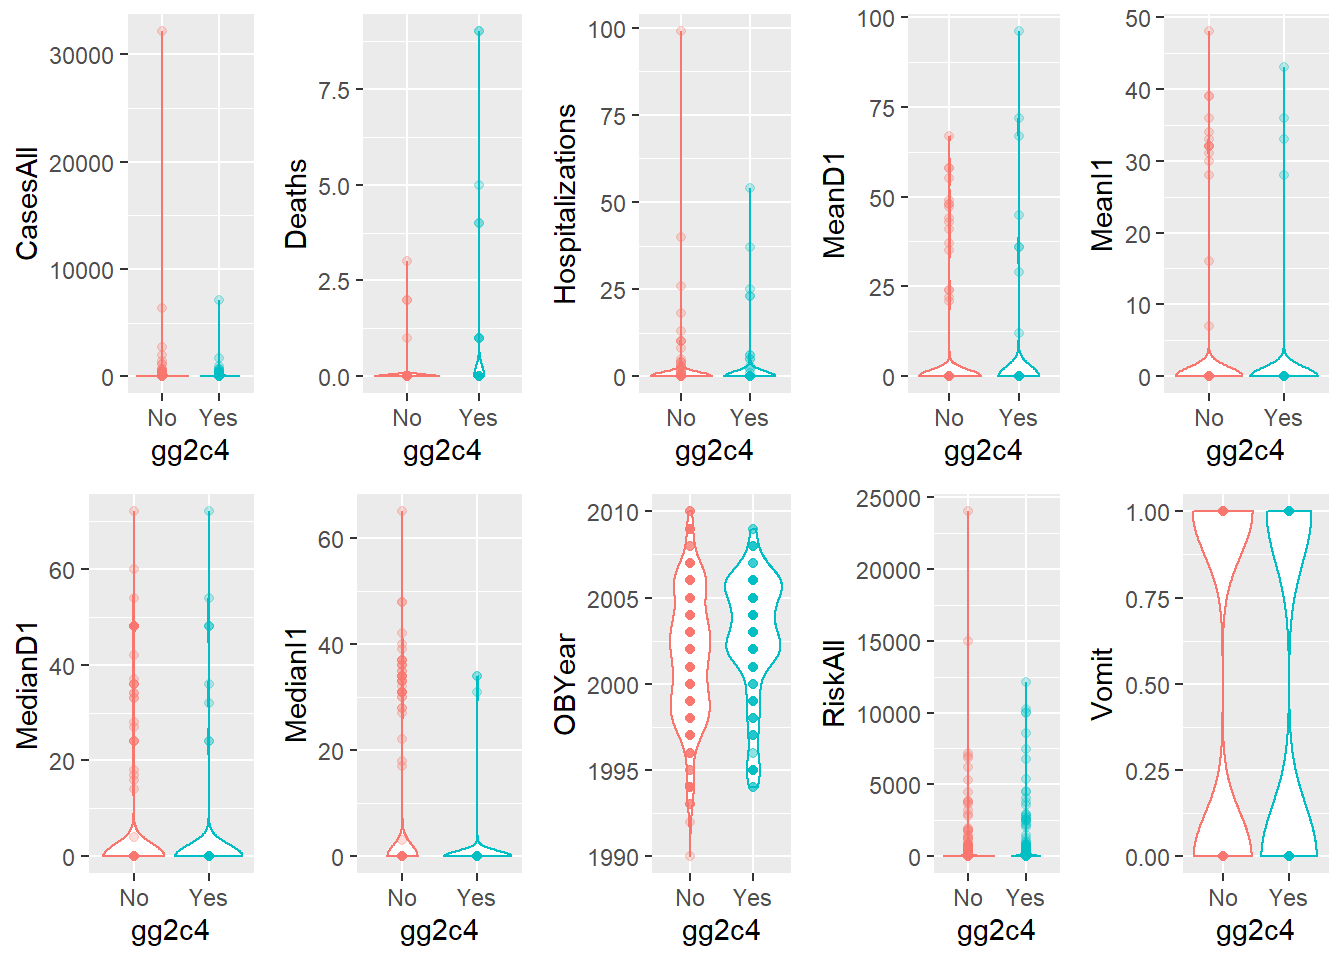
\includegraphics{Variable_Selection_files/figure-latex/plots-1-1.pdf}

Things look ok, apart from the skew in the predictors we discussed
previously.

Next, let's create plots for the categorical variabless. You can use for
instance \texttt{geom\_count} for it, or some other representation. If
you prefer lots of tables, that's ok too.

\begin{Shaded}
\begin{Highlighting}[]
\CommentTok{#write code that produces plots or tables showing our outcome of interest and each categorical predictor.}


\NormalTok{gg2c4_vs_action1 <-}\StringTok{ }\NormalTok{CompData }\OperatorTok\StringTok{ }

\StringTok{  }\KeywordTok{ggplot}\NormalTok{(}\KeywordTok{aes}\NormalTok{(}\DataTypeTok{x =}\NormalTok{ gg2c4, }\DataTypeTok{y =}\NormalTok{ Action1)) }\OperatorTok{+}\StringTok{ }

\StringTok{  }\KeywordTok{geom_count}\NormalTok{() }



\NormalTok{gg2c4_vs_country <-}\StringTok{ }\NormalTok{CompData }\OperatorTok\StringTok{ }

\StringTok{  }\KeywordTok{ggplot}\NormalTok{(}\KeywordTok{aes}\NormalTok{(}\DataTypeTok{x =}\NormalTok{ gg2c4, }\DataTypeTok{y =}\NormalTok{ Country)) }\OperatorTok{+}\StringTok{ }

\StringTok{  }\KeywordTok{geom_count}\NormalTok{() }



\NormalTok{gg2c4_vs_hemi <-}\StringTok{ }\NormalTok{CompData }\OperatorTok\StringTok{ }

\StringTok{  }\KeywordTok{ggplot}\NormalTok{(}\KeywordTok{aes}\NormalTok{(}\DataTypeTok{x =}\NormalTok{ gg2c4, }\DataTypeTok{y =}\NormalTok{ Hemisphere)) }\OperatorTok{+}\StringTok{ }

\StringTok{  }\KeywordTok{geom_count}\NormalTok{() }



\NormalTok{gg2c4_vs_path1 <-}\StringTok{ }\NormalTok{CompData }\OperatorTok\StringTok{ }

\StringTok{  }\KeywordTok{ggplot}\NormalTok{(}\KeywordTok{aes}\NormalTok{(}\DataTypeTok{x =}\NormalTok{ gg2c4, }\DataTypeTok{y =}\NormalTok{ Path1)) }\OperatorTok{+}\StringTok{ }

\StringTok{  }\KeywordTok{geom_count}\NormalTok{() }

\KeywordTok{grid.arrange}\NormalTok{(gg2c4_vs_action1, gg2c4_vs_country, gg2c4_vs_hemi, gg2c4_vs_path1, }\DataTypeTok{nrow =} \DecValTok{2}\NormalTok{)}
\end{Highlighting}
\end{Shaded}

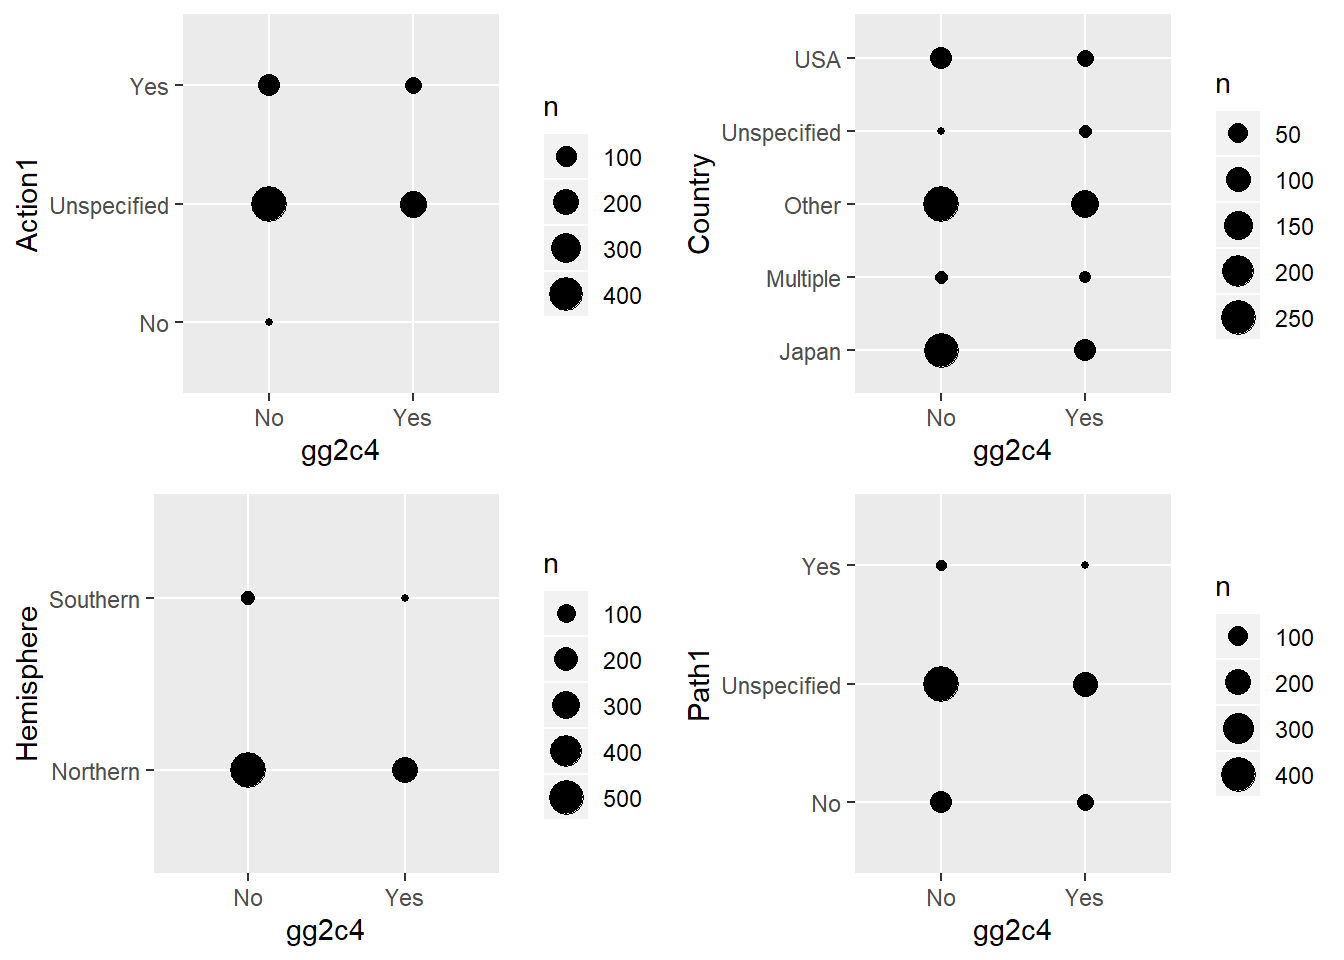
\includegraphics{Variable_Selection_files/figure-latex/plots-2-1.pdf}

\begin{Shaded}
\begin{Highlighting}[]
\NormalTok{gg2c4_vs_season <-}\StringTok{ }\NormalTok{CompData }\OperatorTok\StringTok{ }

\StringTok{  }\KeywordTok{ggplot}\NormalTok{(}\KeywordTok{aes}\NormalTok{(}\DataTypeTok{x =}\NormalTok{ gg2c4, }\DataTypeTok{y =}\NormalTok{ season)) }\OperatorTok{+}\StringTok{ }

\StringTok{  }\KeywordTok{geom_count}\NormalTok{() }



\NormalTok{gg2c4_vs_tras1 <-}\StringTok{ }\NormalTok{CompData }\OperatorTok\StringTok{ }

\StringTok{  }\KeywordTok{ggplot}\NormalTok{(}\KeywordTok{aes}\NormalTok{(}\DataTypeTok{x =}\NormalTok{ gg2c4, }\DataTypeTok{y =}\NormalTok{ Trans1)) }\OperatorTok{+}\StringTok{ }

\StringTok{  }\KeywordTok{geom_count}\NormalTok{() }



\NormalTok{gg2c4_vs_Setting <-}\StringTok{ }\NormalTok{CompData }\OperatorTok\StringTok{ }

\StringTok{  }\KeywordTok{ggplot}\NormalTok{(}\KeywordTok{aes}\NormalTok{(}\DataTypeTok{x =}\NormalTok{ gg2c4, }\DataTypeTok{y =}\NormalTok{ Action1)) }\OperatorTok{+}\StringTok{ }

\StringTok{  }\KeywordTok{geom_count}\NormalTok{() }



\KeywordTok{grid.arrange}\NormalTok{(gg2c4_vs_season, gg2c4_vs_tras1, gg2c4_vs_Setting, }\DataTypeTok{nrow =} \DecValTok{2}\NormalTok{)}
\end{Highlighting}
\end{Shaded}

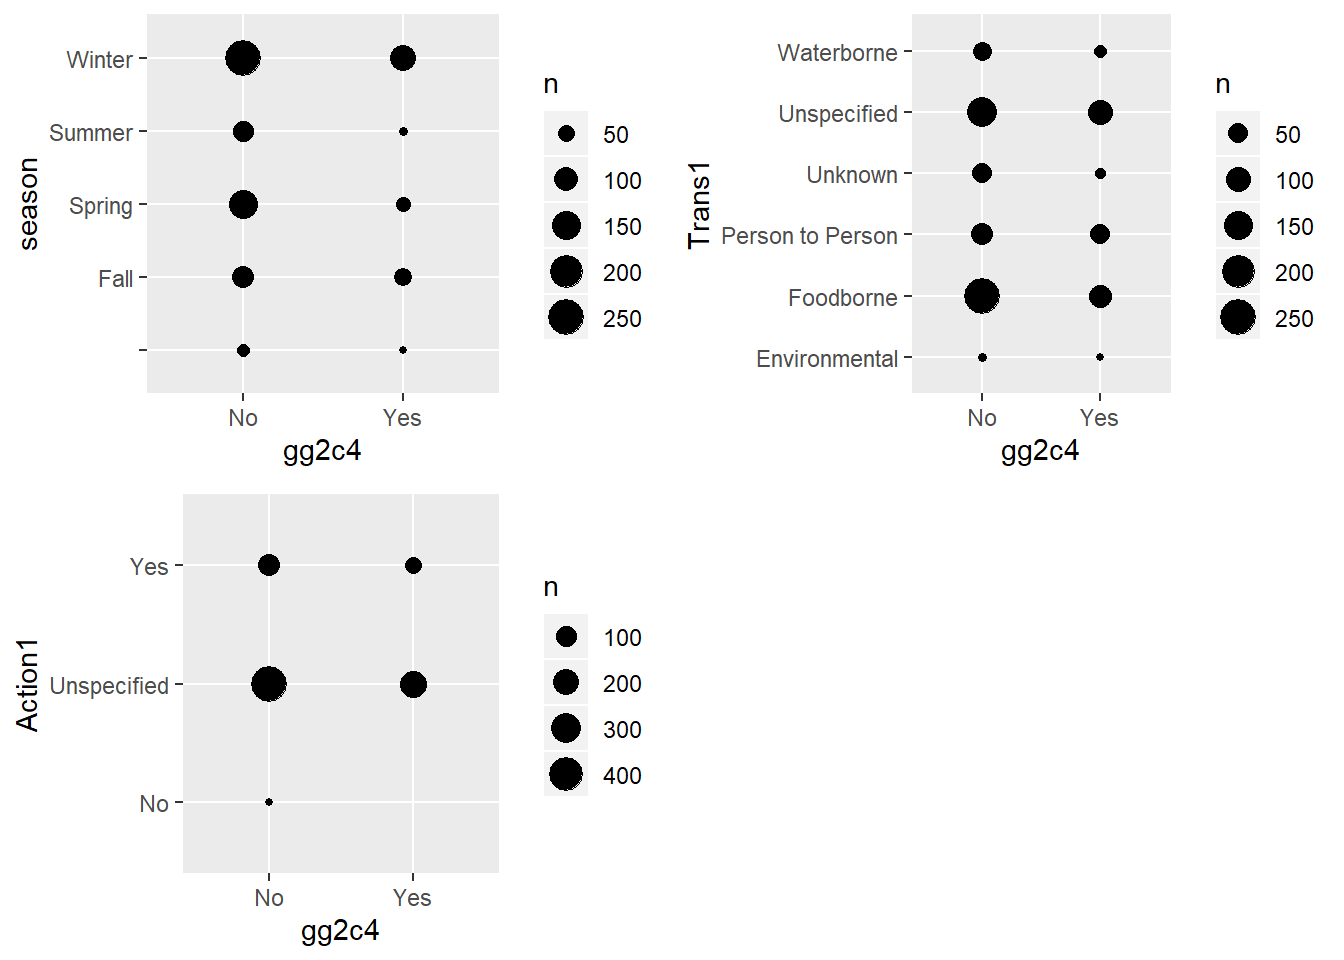
\includegraphics{Variable_Selection_files/figure-latex/unnamed-chunk-1-1.pdf}

You should see from plots or tables that some of the categories are
small, e.g.~for Action1, the ``No'' category is very small. Very few
entries for a given factor create problems during cross-validation
(since we can't have a level show up in the holdout if it wasn't part of
the fitting set). So let's look at those factor variables a bit closer
and fix as needed.

\begin{Shaded}
\begin{Highlighting}[]
\CommentTok{#write code that looks at tables/summaries of factors }


\KeywordTok{summary}\NormalTok{(CompData)}
\end{Highlighting}
\end{Shaded}

\begin{verbatim}
##         Action1       CasesAll            Country        Deaths       
##  No         :  1   Min.   :    1   Other      :408   Min.   :0.00000  
##  Unspecified:677   1st Qu.:    9   Japan      :316   1st Qu.:0.00000  
##  Yes        :172   Median :   25   USA        : 98   Median :0.00000  
##                    Mean   :  128   Multiple   : 16   Mean   :0.05176  
##                    3rd Qu.:   65   Unspecified: 12   3rd Qu.:0.00000  
##                    Max.   :32150   Australia  :  0   Max.   :9.00000  
##                                    (Other)    :  0                    
##  gg2c4           Hemisphere  Hospitalizations      MeanD1      
##  No :591   Northern   :798   Min.   : 0.0000   Min.   : 0.000  
##  Yes:259   Southern   : 52   1st Qu.: 0.0000   1st Qu.: 0.000  
##            Unspecified:  0   Median : 0.0000   Median : 0.000  
##                              Mean   : 0.5518   Mean   : 1.311  
##                              3rd Qu.: 0.0000   3rd Qu.: 0.000  
##                              Max.   :99.0000   Max.   :96.000  
##                                                                
##      MeanI1           MedianD1         MedianI1          OBYear    
##  Min.   : 0.0000   Min.   : 0.000   Min.   : 0.000   Min.   :1990  
##  1st Qu.: 0.0000   1st Qu.: 0.000   1st Qu.: 0.000   1st Qu.:1999  
##  Median : 0.0000   Median : 0.000   Median : 0.000   Median :2002  
##  Mean   : 0.7165   Mean   : 2.312   Mean   : 1.722   Mean   :2002  
##  3rd Qu.: 0.0000   3rd Qu.: 0.000   3rd Qu.: 0.000   3rd Qu.:2005  
##  Max.   :48.0000   Max.   :72.000   Max.   :65.000   Max.   :2010  
##                                                                    
##          Path1        RiskAll           season                 Trans1   
##  No         :196   Min.   :    0.0         : 56   Environmental   : 11  
##  Unspecified:614   1st Qu.:    0.0   Fall  :135   Foodborne       :337  
##  Yes        : 40   Median :   21.5   Spring:187   Person to Person:119  
##                    Mean   :  359.7   Summer:102   Unknown         : 61  
##                    3rd Qu.:  112.0   Winter:370   Unspecified     :261  
##                    Max.   :24000.0                Waterborne      : 61  
##                                                                         
##      Vomit              Setting   
##  Min.   :0.0000   Other     :682  
##  1st Qu.:0.0000   Restaurant:168  
##  Median :0.0000                   
##  Mean   :0.4894                   
##  3rd Qu.:1.0000                   
##  Max.   :1.0000                   
## 
\end{verbatim}

\begin{Shaded}
\begin{Highlighting}[]
\KeywordTok{table}\NormalTok{(CompData}\OperatorTok{$}\NormalTok{Action1)}
\end{Highlighting}
\end{Shaded}

\begin{verbatim}
## 
##          No Unspecified         Yes 
##           1         677         172
\end{verbatim}

\begin{Shaded}
\begin{Highlighting}[]
\KeywordTok{table}\NormalTok{(CompData}\OperatorTok{$}\NormalTok{Country)}
\end{Highlighting}
\end{Shaded}

\begin{verbatim}
## 
##   Australia     Austria      Brazil       Ca da        Chi      Croatia 
##           0           0           0           0           0           0 
##     Denmark      France        Iraq      Israel       Italy       Japan 
##           0           0           0           0           0         316 
##    Multiple Netherlands New Zealand      Norway       Other    Scotland 
##          16           0           0           0         408           0 
##       Spain          UK Unspecified         USA 
##           0           0          12          98
\end{verbatim}

\begin{Shaded}
\begin{Highlighting}[]
\KeywordTok{table}\NormalTok{(CompData}\OperatorTok{$}\NormalTok{Trans1)}
\end{Highlighting}
\end{Shaded}

\begin{verbatim}
## 
##    Environmental        Foodborne Person to Person          Unknown 
##               11              337              119               61 
##      Unspecified       Waterborne 
##              261               61
\end{verbatim}

You should see from your explorations above that there is only a single
entry for \emph{No} in \texttt{Action1}, and small entries for
\emph{Multiple} and \emph{Unspecified} in \texttt{Country} and
\emph{Environmental} in \texttt{Trans1}. The single \emph{No} should be
fixed, the other somewhat small groupings might be ok. It depends on
scientific rationale and method of analysis if you should modify/group
those or not. We'll do that.

Change things as follows: Remove the observation for which action is
\emph{No}, combine Countries into 3 groups Japan/USA/Other, and since I
don't even know what biologically the difference is between
\emph{Environmental} and \emph{Waterborne} transmission (seems the same
route to me based on my norovirus knowledge), we'll move the Waterborne
into the environmental. Finally, I noticed there is a blank category for
season. That likely means it wasn't stated in the paper. Let's recode
that as \emph{Unknown}. Finally, re-order data such that the outcome is
the first column and again remove empty factor levels. Then look at your
resulting data frame.

\begin{Shaded}
\begin{Highlighting}[]
\CommentTok{#write code that does the actions described above}
\CommentTok{#remove no}
\NormalTok{remove_no <-}\StringTok{ }\NormalTok{CompData }\OperatorTok

\StringTok{  }\KeywordTok{subset}\NormalTok{(Action1 }\OperatorTok{!=}\StringTok{ "No"}\NormalTok{)}

\NormalTok{remove_no <-}\StringTok{ }\NormalTok{remove_no }\OperatorTok

\StringTok{  }\KeywordTok{droplevels}\NormalTok{(remove_no}\OperatorTok{$}\NormalTok{Action1)}

\KeywordTok{summary}\NormalTok{(remove_no}\OperatorTok{$}\NormalTok{Action1)}
\end{Highlighting}
\end{Shaded}

\begin{verbatim}
## Unspecified         Yes 
##         677         172
\end{verbatim}

\begin{Shaded}
\begin{Highlighting}[]
\CommentTok{#recode country}

\KeywordTok{summary}\NormalTok{(remove_no}\OperatorTok{$}\NormalTok{Country)}
\end{Highlighting}
\end{Shaded}

\begin{verbatim}
##   Australia     Austria      Brazil       Ca da        Chi      Croatia 
##           0           0           0           0           0           0 
##     Denmark      France        Iraq      Israel       Italy       Japan 
##           0           0           0           0           0         316 
##    Multiple Netherlands New Zealand      Norway       Other    Scotland 
##          16           0           0           0         408           0 
##       Spain          UK Unspecified         USA 
##           0           0          11          98
\end{verbatim}

\begin{Shaded}
\begin{Highlighting}[]
\NormalTok{Multiple<-}\StringTok{ }\NormalTok{remove_no }\OperatorTok

\StringTok{  }\KeywordTok{mutate}\NormalTok{(}\DataTypeTok{Country=} \KeywordTok{fct_recode}\NormalTok{(Country, }\StringTok{"Other"}\NormalTok{ =}\StringTok{ "Multiple"}\NormalTok{))}

         

\NormalTok{Unspec <-}\StringTok{ }\NormalTok{Multiple }\OperatorTok

\StringTok{  }\KeywordTok{mutate}\NormalTok{(}\DataTypeTok{Country=} \KeywordTok{fct_recode}\NormalTok{(Country, }\StringTok{"Other"}\NormalTok{ =}\StringTok{ "Unspecified"}\NormalTok{))}


\KeywordTok{summary}\NormalTok{(Unspec}\OperatorTok{$}\NormalTok{Country)}
\end{Highlighting}
\end{Shaded}

\begin{verbatim}
##   Australia     Austria      Brazil       Ca da        Chi      Croatia 
##           0           0           0           0           0           0 
##     Denmark      France        Iraq      Israel       Italy       Japan 
##           0           0           0           0           0         316 
##       Other Netherlands New Zealand      Norway    Scotland       Spain 
##         435           0           0           0           0           0 
##          UK         USA 
##           0          98
\end{verbatim}

\begin{Shaded}
\begin{Highlighting}[]
\KeywordTok{summary}\NormalTok{(Unspec}\OperatorTok{$}\NormalTok{Trans1)}
\end{Highlighting}
\end{Shaded}

\begin{verbatim}
##    Environmental        Foodborne Person to Person          Unknown 
##               11              337              119               61 
##      Unspecified       Waterborne 
##              260               61
\end{verbatim}

\begin{Shaded}
\begin{Highlighting}[]
\CommentTok{#environemntal}


\NormalTok{Environmental <-}\StringTok{ }\NormalTok{Unspec }\OperatorTok

\StringTok{  }\KeywordTok{mutate}\NormalTok{(}\DataTypeTok{Trans1=} \KeywordTok{fct_recode}\NormalTok{(Trans1, }\StringTok{"Environmental"}\NormalTok{ =}\StringTok{ "Waterborne"}\NormalTok{))}

\KeywordTok{summary}\NormalTok{(Environmental}\OperatorTok{$}\NormalTok{Trans1)}
\end{Highlighting}
\end{Shaded}

\begin{verbatim}
##    Environmental        Foodborne Person to Person          Unknown 
##               72              337              119               61 
##      Unspecified 
##              260
\end{verbatim}

\begin{Shaded}
\begin{Highlighting}[]
\CommentTok{#Seasons}

\KeywordTok{summary}\NormalTok{(Environmental}\OperatorTok{$}\NormalTok{season)}
\end{Highlighting}
\end{Shaded}

\begin{verbatim}
##          Fall Spring Summer Winter 
##     55    135    187    102    370
\end{verbatim}

\begin{Shaded}
\begin{Highlighting}[]
\NormalTok{Season <-}\StringTok{ }\NormalTok{Environmental }\OperatorTok

\StringTok{  }\KeywordTok{mutate}\NormalTok{(}\DataTypeTok{season=} \KeywordTok{fct_recode}\NormalTok{(season, }\StringTok{"Unknown"}\NormalTok{ =}\StringTok{ ""}\NormalTok{))}

\KeywordTok{summary}\NormalTok{(Season}\OperatorTok{$}\NormalTok{season)}
\end{Highlighting}
\end{Shaded}

\begin{verbatim}
## Unknown    Fall  Spring  Summer  Winter 
##      55     135     187     102     370
\end{verbatim}

\begin{Shaded}
\begin{Highlighting}[]
\CommentTok{#reorder outcome}
\NormalTok{Outcomefirst <-}\StringTok{ }\NormalTok{Season }\OperatorTok

\StringTok{  }\KeywordTok{select}\NormalTok{(gg2c4, }\KeywordTok{everything}\NormalTok{())}

\KeywordTok{summary}\NormalTok{(Outcomefirst)}
\end{Highlighting}
\end{Shaded}

\begin{verbatim}
##  gg2c4            Action1       CasesAll            Country   
##  No :590   Unspecified:677   Min.   :    1.0   Other    :435  
##  Yes:259   Yes        :172   1st Qu.:    9.0   Japan    :316  
##                              Median :   25.0   USA      : 98  
##                              Mean   :  128.1   Australia:  0  
##                              3rd Qu.:   65.0   Austria  :  0  
##                              Max.   :32150.0   Brazil   :  0  
##                                                (Other)  :  0  
##      Deaths           Hemisphere  Hospitalizations      MeanD1      
##  Min.   :0.00000   Northern:797   Min.   : 0.0000   Min.   : 0.000  
##  1st Qu.:0.00000   Southern: 52   1st Qu.: 0.0000   1st Qu.: 0.000  
##  Median :0.00000                  Median : 0.0000   Median : 0.000  
##  Mean   :0.05183                  Mean   : 0.5524   Mean   : 1.312  
##  3rd Qu.:0.00000                  3rd Qu.: 0.0000   3rd Qu.: 0.000  
##  Max.   :9.00000                  Max.   :99.0000   Max.   :96.000  
##                                                                     
##      MeanI1           MedianD1         MedianI1          OBYear    
##  Min.   : 0.0000   Min.   : 0.000   Min.   : 0.000   Min.   :1990  
##  1st Qu.: 0.0000   1st Qu.: 0.000   1st Qu.: 0.000   1st Qu.:1999  
##  Median : 0.0000   Median : 0.000   Median : 0.000   Median :2002  
##  Mean   : 0.7173   Mean   : 2.314   Mean   : 1.724   Mean   :2002  
##  3rd Qu.: 0.0000   3rd Qu.: 0.000   3rd Qu.: 0.000   3rd Qu.:2005  
##  Max.   :48.0000   Max.   :72.000   Max.   :65.000   Max.   :2010  
##                                                                    
##          Path1        RiskAll            season                 Trans1   
##  No         :196   Min.   :    0.0   Unknown: 55   Environmental   : 72  
##  Unspecified:613   1st Qu.:    0.0   Fall   :135   Foodborne       :337  
##  Yes        : 40   Median :   22.0   Spring :187   Person to Person:119  
##                    Mean   :  360.1   Summer :102   Unknown         : 61  
##                    3rd Qu.:  112.0   Winter :370   Unspecified     :260  
##                    Max.   :24000.0                                       
##                                                                          
##      Vomit              Setting   
##  Min.   :0.0000   Other     :681  
##  1st Qu.:0.0000   Restaurant:168  
##  Median :0.0000                   
##  Mean   :0.4888                   
##  3rd Qu.:1.0000                   
##  Max.   :1.0000                   
## 
\end{verbatim}

\begin{Shaded}
\begin{Highlighting}[]
\KeywordTok{vis_dat}\NormalTok{(Outcomefirst)}
\end{Highlighting}
\end{Shaded}

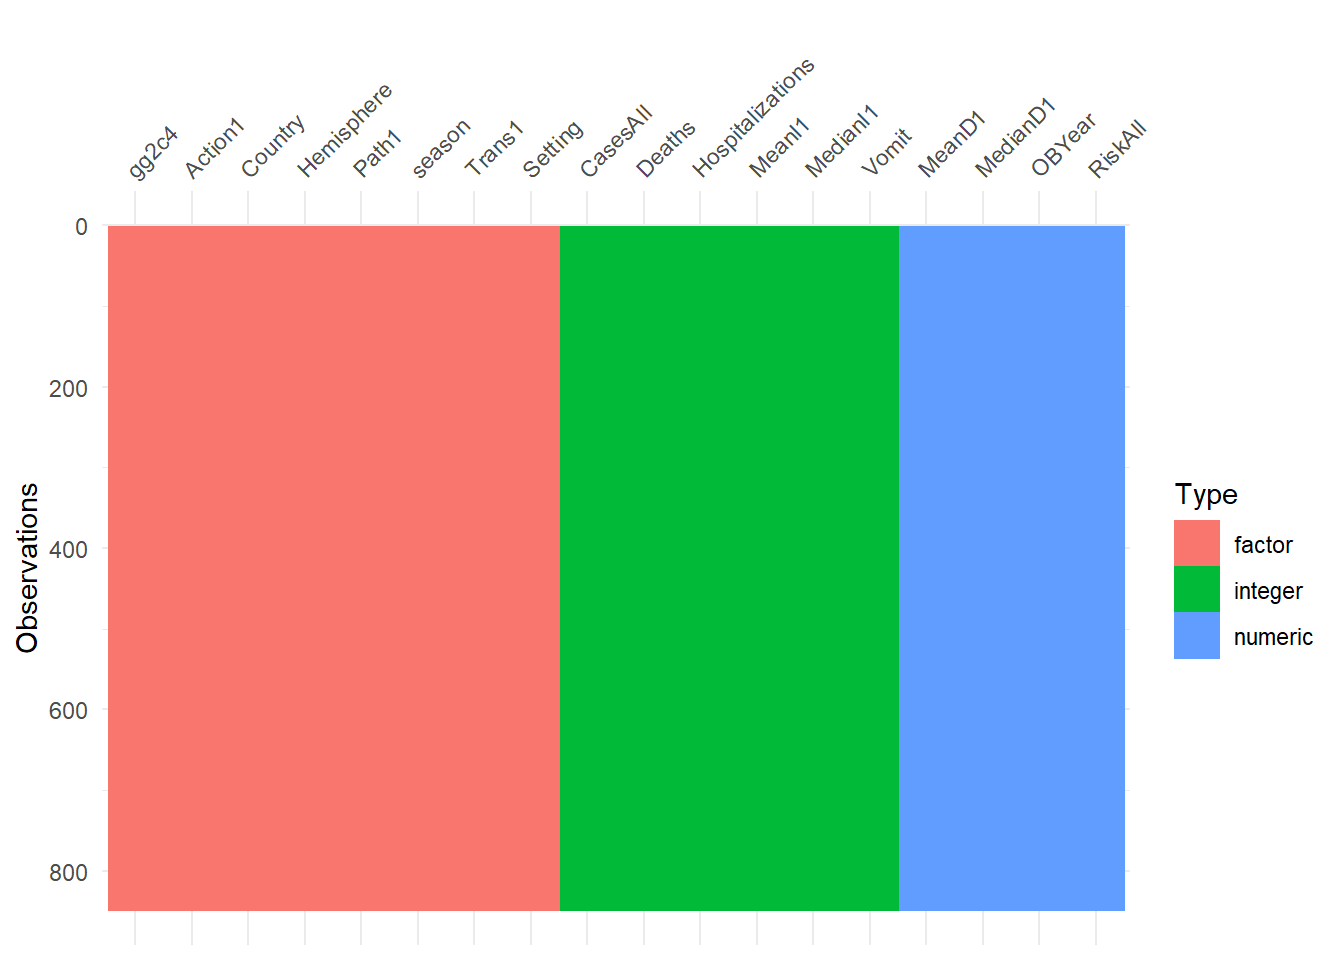
\includegraphics{Variable_Selection_files/figure-latex/more-factor-cleaning-1.pdf}

At this step, you should have a dataframe containing 850 observations,
and 18 variables: 1 outcome, 9 numeric/integer predictors, and 8 factor
variables. There should be no missing values. The outcome,
\texttt{gg2c4}, should be in the 1st slot.

\hypertarget{data-splitting}{%
\section{Data splitting}\label{data-splitting}}

We could do data splitting again as we did in the previous exercise, to
have a final test set. But since you saw how it works in the previous
exercise, we skip it here. We use the full data to fit to our models.
We'll still use cross-validation to get a more honest estimate of model
performance. For a real data analysis, the choice to keep some for a
final test or not is based on your goals. If your focus is predictive
performance, you should consider this split. If your focus is inference
or exploratory analysis, you might want to skip this.

\hypertarget{model-fitting}{%
\section{Model fitting}\label{model-fitting}}

So I had planned to use \texttt{caret} exclusivley for this course. Last
time I tried feature/subset selection with \texttt{caret}, I found it
buggy and not too well documented. I had hoped this had improved since.
Unortunately, I was again not really able to get things to work. So even
though I said we likely won't use the \texttt{mlr} package, I decided
that to be able to nicely practice feature/subset selection, we need to
do so. It's not a bad idea to get familiar with that package, at times
\texttt{caret} can do things \texttt{mlr} can't do and the reverse. So
knowing how to use both is good. We'll thus use \texttt{mlr} to do our
model fitting in this exercise.

\hypertarget{parallelization}{%
\section{Parallelization}\label{parallelization}}

\texttt{mlr} allows you to run things in parallel by using multiple
cores (\texttt{caret} does too). For instance, if you do 5x
cross-validation 5x repeated, you essentially run a very similar piece
of code 25 times. Normally, you would run one at a time. But if you have
it on a machine with 25 cores, all those 25 could run at the same time,
giving you a speed-up of 25 (or close to, there is usually some overhead
related to doing things in parallel). This kind of parallel computing is
sometimes called \emph{embarassingly parallel}, because it's so
embarassingly simple to split the task into parallel streams.

Since doing the subset selection below starts getting slow, and because
it's a good topic to know about, we are going to use parallelization
here. \texttt{mlr} uses the package \texttt{parallelMap} for this. All
you need to do is specify the number of cores/processors you want to use
and start the parallel system, and \texttt{mlr} then automatically does
things in parallel if feasible.

\begin{Shaded}
\begin{Highlighting}[]
\CommentTok{#set the number of cores you want to use. Note that this is actually the number of 'logical processors', which is 2x the number of cores. On a windows machine, the number of cores/logical processors can be found in the task manager. You should only set it to what your computer has (or less). So if your computer has say 4 or 6 cores, you can set it to that, or some lower number. Setting it to a number higher than the cores your computer has doesn't further speed up things, in fact it slows things down.}
\NormalTok{ncpu=}\DecValTok{4}\NormalTok{;}
\CommentTok{#if you don't want to run things in parallel, or don't have multiple cores (unlikely nowadays), }
\CommentTok{#just comment out the line below.}
\KeywordTok{parallelStartSocket}\NormalTok{(ncpu, }\DataTypeTok{show.info=}\OtherTok{FALSE}\NormalTok{) }
\end{Highlighting}
\end{Shaded}

\hypertarget{setup}{%
\section{Setup}\label{setup}}

Some setup settings that are used in various code chunks below.

\begin{Shaded}
\begin{Highlighting}[]
\NormalTok{outcome <-}\StringTok{ }\NormalTok{Outcomefirst}\OperatorTok{$}\NormalTok{gg2c4 }
\NormalTok{outcomename =}\StringTok{ "gg2c4"}
\NormalTok{predictors <-}\StringTok{ }\NormalTok{Outcomefirst[,}\OperatorTok{-}\DecValTok{1}\NormalTok{]}
\NormalTok{npred=}\KeywordTok{ncol}\NormalTok{(predictors)}
\CommentTok{#set sampling method for performance evaluation}
\CommentTok{#here, we use 5-fold cross-validation, 5-times repeated}
\NormalTok{sampling_choice =}\StringTok{ }\KeywordTok{makeResampleDesc}\NormalTok{(}\StringTok{"RepCV"}\NormalTok{, }\DataTypeTok{reps =} \DecValTok{5}\NormalTok{, }\DataTypeTok{folds =} \DecValTok{5}\NormalTok{)}
\end{Highlighting}
\end{Shaded}

\hypertarget{a-null-model}{%
\subsection{A null model}\label{a-null-model}}

To define a null model, we need to determine what performance measure we
want to track. As mentioned in the course materials, there are different
performance measures. Accuracy or misclassification error is simple, it
just counts the number of times the model got it right/wrong. We'll
start with that one, and then try another one later. \texttt{mlr} allows
for a lot of different performance measures for both categorical and
continuous outcomes, see
\href{https://mlr.mlr-org.com/articles/tutorial/performance.html}{here}
and
\href{https://mlr.mlr-org.com/articles/tutorial/measures.html}{here}.

For accuracy, the simplest null model always predicts the most frequent
category. We can use that as baseline performance.

\begin{Shaded}
\begin{Highlighting}[]
\CommentTok{#write code that computes accuracy for a null model}
\CommentTok{#the null model always predicts "No"}
\KeywordTok{measureACC}\NormalTok{(}\StringTok{"No"}\NormalTok{, Outcomefirst}\OperatorTok{$}\NormalTok{gg2c4)}
\end{Highlighting}
\end{Shaded}

\begin{verbatim}
## [1] 0.6949352
\end{verbatim}

You should find that the null model has an accuracy of around 0.69.

\hypertarget{single-predictor-models}{%
\subsection{Single predictor models}\label{single-predictor-models}}

Now let's consider single predictor models, i.e.~we'll fit the outcome
to each predictor one at a time to get an idea of the importance of
individual predictors. To evaluate our model performance, we will use
cross-validation. Since our outcome is categorical, we'll use a logistic
model.

\begin{Shaded}
\begin{Highlighting}[]
\KeywordTok{set.seed}\NormalTok{(}\DecValTok{1111}\NormalTok{) }\CommentTok{#makes each code block reproducible}
\CommentTok{#set learner/model. this corresponds to a logistic model.}
\CommentTok{#mlr calls different models different "learners"}
\NormalTok{learner_name =}\StringTok{ "classif.binomial"}\NormalTok{;}
\NormalTok{mylearner =}\StringTok{ }\KeywordTok{makeLearner}\NormalTok{(learner_name, }\DataTypeTok{predict.type =} \StringTok{"prob"}\NormalTok{)}
\CommentTok{# this will contain the results}
\NormalTok{unifmat=}\KeywordTok{data.frame}\NormalTok{(}\DataTypeTok{variable =} \KeywordTok{rep}\NormalTok{(}\DecValTok{0}\NormalTok{,npred), }\DataTypeTok{Accuracy =} \KeywordTok{rep}\NormalTok{(}\DecValTok{0}\NormalTok{,npred))}
\CommentTok{# loop over each predictor, build simple dataset with just outcome and that predictor, fit it to a glm/logistic model}
\ControlFlowTok{for}\NormalTok{ (nn }\ControlFlowTok{in} \DecValTok{1}\OperatorTok{:}\NormalTok{npred)}
\NormalTok{\{}
\NormalTok{    unidata =}\StringTok{ }\KeywordTok{data.frame}\NormalTok{(}\DataTypeTok{gg2c4 =}\NormalTok{ outcome, Outcomefirst[,nn}\OperatorTok{+}\DecValTok{1}\NormalTok{] )}
    \CommentTok{## Generate the task, i.e. define outcome and predictors to be fit}
\NormalTok{    mytask =}\StringTok{ }\KeywordTok{makeClassifTask}\NormalTok{(}\DataTypeTok{id=}\StringTok{'unianalysis'}\NormalTok{, }\DataTypeTok{data =}\NormalTok{ unidata, }\DataTypeTok{target =}\NormalTok{ outcomename, }\DataTypeTok{positive =} \StringTok{"Yes"}\NormalTok{)}
\NormalTok{    model =}\StringTok{ }\KeywordTok{resample}\NormalTok{(mylearner, }\DataTypeTok{task =}\NormalTok{ mytask, }\DataTypeTok{resampling =}\NormalTok{ sampling_choice, }\DataTypeTok{show.info =} \OtherTok{FALSE}\NormalTok{, }\DataTypeTok{measures =}\NormalTok{ acc )}
\NormalTok{    unifmat[nn,}\DecValTok{1}\NormalTok{] =}\StringTok{ }\KeywordTok{names}\NormalTok{(predictors)[nn] }
\NormalTok{    unifmat[nn,}\DecValTok{2}\NormalTok{] =}\StringTok{ }\NormalTok{model}\OperatorTok{$}\NormalTok{aggr}
\NormalTok{\}}
\KeywordTok{kable}\NormalTok{(unifmat)}
\end{Highlighting}
\end{Shaded}

\begin{longtable}[]{@{}lr@{}}
\toprule
variable & Accuracy\tabularnewline
\midrule
\endhead
Action1 & 0.6949419\tabularnewline
CasesAll & 0.6932711\tabularnewline
Country & 0.6949447\tabularnewline
Deaths & 0.6977905\tabularnewline
Hemisphere & 0.6949502\tabularnewline
Hospitalizations & 0.6941998\tabularnewline
MeanD1 & 0.6946940\tabularnewline
MeanI1 & 0.6949419\tabularnewline
MedianD1 & 0.6949516\tabularnewline
MedianI1 & 0.6949488\tabularnewline
OBYear & 0.6941970\tabularnewline
Path1 & 0.6949279\tabularnewline
RiskAll & 0.6956408\tabularnewline
season & 0.6930609\tabularnewline
Trans1 & 0.6949377\tabularnewline
Vomit & 0.6949572\tabularnewline
Setting & 0.6949126\tabularnewline
\bottomrule
\end{longtable}

So looks like none of the single predictor models have a higher accuracy
than the null. Maybe surprising. We'll get back to that below.

\hypertarget{full-model}{%
\section{Full model}\label{full-model}}

Now let's fit a full logistic model with all predictors.

\begin{Shaded}
\begin{Highlighting}[]
\KeywordTok{set.seed}\NormalTok{(}\DecValTok{1111}\NormalTok{) }\CommentTok{#makes each code block reproducible}
\CommentTok{#do full model with Cross-Validation - to get an idea for the amount of over-fitting a full model does}
\NormalTok{mytask =}\StringTok{ }\KeywordTok{makeClassifTask}\NormalTok{(}\DataTypeTok{id=}\StringTok{'fullanalysis'}\NormalTok{, }\DataTypeTok{data =}\NormalTok{ Outcomefirst, }\DataTypeTok{target =}\NormalTok{ outcomename, }\DataTypeTok{positive =} \StringTok{"Yes"}\NormalTok{)}
\end{Highlighting}
\end{Shaded}

\begin{verbatim}
## Warning in makeTask(type = type, data = data, weights = weights, blocking =
## blocking, : Empty factor levels were dropped for columns: Country
\end{verbatim}

\begin{Shaded}
\begin{Highlighting}[]
\NormalTok{fullmodel =}\StringTok{ }\KeywordTok{resample}\NormalTok{(mylearner, }\DataTypeTok{task =}\NormalTok{ mytask, }\DataTypeTok{resampling =}\NormalTok{ sampling_choice, }\DataTypeTok{show.info =} \OtherTok{FALSE}\NormalTok{, }\DataTypeTok{measures =}\NormalTok{ acc )}
\NormalTok{ACC_fullmodel =}\StringTok{ }\NormalTok{fullmodel}\OperatorTok{$}\NormalTok{aggr[}\DecValTok{1}\NormalTok{]}
\KeywordTok{print}\NormalTok{(ACC_fullmodel)}
\end{Highlighting}
\end{Shaded}

\begin{verbatim}
## acc.test.mean 
##     0.7060188
\end{verbatim}

So a very small improvement over the simple models.

Now let's do subset selection. The code below does it several ways. It
does regular forward and backward selection and floating versions of
those. It also uses a genetic algorithm for selection. See the
\texttt{mlr} website
\href{https://mlr.mlr-org.com/articles/tutorial/feature_selection.html}{here}
for details.

Also note that I included a kind of timer in the code, to see how long
things take. That's a good idea if you run bigger models. You first run
a few iterations on maybe a few cores, then you can compute how long it
would take if you doubled the iterations, or doubled the cores, etc.
This prevents bad surprises of trying to \emph{quickly} run a piece of
code and waiting hours. You should always use short runs to make sure
everything works in principle, and only at the end do the real, long
``production'' runs. Otherwise you might waste hours/days/weeks waiting
for results only to realize that you made a basic mistake and you have
to do it all over.

\begin{Shaded}
\begin{Highlighting}[]
\KeywordTok{set.seed}\NormalTok{(}\DecValTok{1111}\NormalTok{) }
\NormalTok{tstart=}\KeywordTok{proc.time}\NormalTok{(); }\CommentTok{#capture current CPU time for timing how long things take}
\CommentTok{#do 2 forms of forward and backward selection, just to compare}
\NormalTok{select_methods=}\KeywordTok{c}\NormalTok{(}\StringTok{"sbs"}\NormalTok{,}\StringTok{"sfbs"}\NormalTok{,}\StringTok{"sfs"}\NormalTok{,}\StringTok{"sffs"}\NormalTok{) }
\NormalTok{resmat=}\KeywordTok{data.frame}\NormalTok{(}\DataTypeTok{method =} \KeywordTok{rep}\NormalTok{(}\DecValTok{0}\NormalTok{,}\DecValTok{4}\NormalTok{), }\DataTypeTok{Accuracy =} \KeywordTok{rep}\NormalTok{(}\DecValTok{0}\NormalTok{,}\DecValTok{4}\NormalTok{), }\DataTypeTok{Model =} \KeywordTok{rep}\NormalTok{(}\DecValTok{0}\NormalTok{,}\DecValTok{4}\NormalTok{))}
\NormalTok{ct=}\DecValTok{1}\NormalTok{;}
\ControlFlowTok{for}\NormalTok{ (select_method }\ControlFlowTok{in}\NormalTok{ select_methods) }\CommentTok{#loop over all stepwise selection methods}
\NormalTok{\{}
\NormalTok{  ctrl =}\StringTok{ }\KeywordTok{makeFeatSelControlSequential}\NormalTok{(}\DataTypeTok{method =}\NormalTok{ select_method)}
  \KeywordTok{print}\NormalTok{(}\KeywordTok{sprintf}\NormalTok{(}\StringTok{'doing subset selection with method %s '}\NormalTok{,select_method))}
\NormalTok{  sfeat_res =}\StringTok{ }\KeywordTok{selectFeatures}\NormalTok{(}\DataTypeTok{learner =}\NormalTok{ mylearner, }
                             \DataTypeTok{task =}\NormalTok{ mytask, }
                             \DataTypeTok{resampling =}\NormalTok{ sampling_choice, }
                             \DataTypeTok{control =}\NormalTok{ ctrl, }
                             \DataTypeTok{show.info =} \OtherTok{FALSE}\NormalTok{,}
                             \DataTypeTok{measures =}\NormalTok{ acc)}
  
\NormalTok{  resmat[ct,}\DecValTok{1}\NormalTok{] =}\StringTok{ }\NormalTok{select_methods[ct]}
\NormalTok{  resmat[ct,}\DecValTok{2}\NormalTok{] =}\StringTok{ }\NormalTok{sfeat_res}\OperatorTok{$}\NormalTok{y}
\NormalTok{  resmat[ct,}\DecValTok{3}\NormalTok{] =}\StringTok{ }\KeywordTok{paste}\NormalTok{(}\KeywordTok{as.vector}\NormalTok{(sfeat_res}\OperatorTok{$}\NormalTok{x), }\DataTypeTok{collapse=} \StringTok{', '}\NormalTok{)}
\NormalTok{  ct=ct}\OperatorTok{+}\DecValTok{1}\NormalTok{;}
\NormalTok{\}}
\end{Highlighting}
\end{Shaded}

\begin{verbatim}
## [1] "doing subset selection with method sbs "
## [1] "doing subset selection with method sfbs "
## [1] "doing subset selection with method sfs "
## [1] "doing subset selection with method sffs "
\end{verbatim}

\begin{Shaded}
\begin{Highlighting}[]
\CommentTok{# do feature selection with genetic algorithm}
\NormalTok{maxit =}\StringTok{ }\DecValTok{100} \CommentTok{#number of iterations - should be large for 'production run'}
\NormalTok{ctrl_GA =}\KeywordTok{makeFeatSelControlGA}\NormalTok{(}\DataTypeTok{maxit =}\NormalTok{ maxit)}
\KeywordTok{print}\NormalTok{(}\KeywordTok{sprintf}\NormalTok{(}\StringTok{'doing subset selection with genetic algorithm'}\NormalTok{))}
\end{Highlighting}
\end{Shaded}

\begin{verbatim}
## [1] "doing subset selection with genetic algorithm"
\end{verbatim}

\begin{Shaded}
\begin{Highlighting}[]
\NormalTok{sfeatga_res =}\StringTok{ }\KeywordTok{selectFeatures}\NormalTok{(}\DataTypeTok{learner =}\NormalTok{ mylearner, }
                                   \DataTypeTok{task =}\NormalTok{ mytask, }
                                   \DataTypeTok{resampling =}\NormalTok{ sampling_choice, }
                                   \DataTypeTok{control =}\NormalTok{ ctrl_GA, }
                                   \DataTypeTok{show.info =} \OtherTok{FALSE}\NormalTok{,}
                                   \DataTypeTok{measures =}\NormalTok{ acc)}
\NormalTok{resmat[}\DecValTok{5}\NormalTok{,}\DecValTok{1}\NormalTok{] =}\StringTok{ "GA"}
\NormalTok{resmat[}\DecValTok{5}\NormalTok{,}\DecValTok{2}\NormalTok{] =}\StringTok{ }\NormalTok{sfeatga_res}\OperatorTok{$}\NormalTok{y}
\NormalTok{resmat[}\DecValTok{5}\NormalTok{,}\DecValTok{3}\NormalTok{] =}\StringTok{ }\KeywordTok{paste}\NormalTok{(}\KeywordTok{as.vector}\NormalTok{(sfeatga_res}\OperatorTok{$}\NormalTok{x), }\DataTypeTok{collapse=} \StringTok{', '}\NormalTok{)}
\NormalTok{runtime.minutes_SS=(}\KeywordTok{proc.time}\NormalTok{()}\OperatorTok{-}\NormalTok{tstart)[[}\DecValTok{3}\NormalTok{]]}\OperatorTok{/}\DecValTok{60}\NormalTok{; }\CommentTok{#total time in minutes the optimization took}
\KeywordTok{print}\NormalTok{(}\KeywordTok{sprintf}\NormalTok{(}\StringTok{'subset selection took %f minutes'}\NormalTok{,runtime.minutes_SS));}
\end{Highlighting}
\end{Shaded}

\begin{verbatim}
## [1] "subset selection took 3.355833 minutes"
\end{verbatim}

\begin{Shaded}
\begin{Highlighting}[]
\KeywordTok{kable}\NormalTok{(resmat)}
\end{Highlighting}
\end{Shaded}

\begin{longtable}[]{@{}lrl@{}}
\toprule
method & Accuracy & Model\tabularnewline
\midrule
\endhead
sbs & 0.7203857 & Action1, Country, Deaths, MedianI1, OBYear, RiskAll,
season, Trans1, Vomit, Setting\tabularnewline
sfbs & 0.7187539 & Action1, Country, Deaths, OBYear, Path1, season,
Trans1, Vomit, Setting\tabularnewline
sfs & 0.6949447 &\tabularnewline
sffs & 0.6949669 &\tabularnewline
GA & 0.7147567 & Action1, CasesAll, Country, Deaths, OBYear, Path1,
RiskAll, season, Trans1, Vomit, Setting\tabularnewline
\bottomrule
\end{longtable}

So we find that some of the sub-models perform somewhat better. Note
that the different methods find different submodels and the forward
selection method seems to fail (since none of the single-predictor
models is better than the null, it stops there). Also note that the
genetic algorithm was only allowed to run for a short time (the number
if iterations is small). To get potentially better results, that should
be increased to a larger number, e.g.~1000 or more. But this will take a
longer time, unless you have many cores you can use when you
parallelize.

\hypertarget{different-performance-measures}{%
\section{Different performance
measures}\label{different-performance-measures}}

So far, we found that some of the sub-models provide a minor improvement
over the simple null or single-predictor models or the full model.
However, the improvement is not much.

We could try tweaking further, e.g.~by pre-processing the predictors
(which is a good idea to try, but we won't do here) or testing a
different model (which we'll do below).

For now, I want to discuss performance measure a bit more. The problem
is that logistic regression, as well as many (though not all) algorithms
that are used for classification (predicting categorical outcomes)
return probabilities for an outcome to belong to a certain category.
Those are then turned into Yes/No predictions (in the case with 2
outcomes like we have here), based on some cut-off. By default, a
probability value of 0.5 is chosen. If the model predicts that there is
a 0.5 or greater probability of the outcome being ``Yes'', it is scored
as such in the prediction, otherwise as no. However, this 0.5 threshold
is not always good. It could be that we might get a much better model if
we use another threshold. There is a technique that scans over different
thresholds and evaluates model performance for each threshold. This is
generally called \emph{receiver operating curve}. If this concept is new
to you, check out
\href{https://en.wikipedia.org/wiki/Receiver_operating_characteristic}{this
article on Wikipedia} or
\href{https://mlr.mlr-org.com/articles/tutorial/roc_analysis.html}{this
tutorial on the mlr website}.

Using this approach, a model is evaluated based on the Area under the
curve (AUC), with an AUC=0.5 meaning a model is not better than chance,
and AUC=1 meaning a perfect model. Let's re-do the analysis above, but
replace accuracy with AUC.

\hypertarget{model-performance-with-auc}{%
\section{Model performance with AUC}\label{model-performance-with-auc}}

\begin{Shaded}
\begin{Highlighting}[]
\CommentTok{#write code that computes AUC for a null model}
\CommentTok{#the null model always predicts "No"}
\CommentTok{#the auc function in the pROC package is useful}
\CommentTok{#or you can use any other package/function you want to use to compute AUC/ROC}


\NormalTok{nullmod <-}\StringTok{ }\KeywordTok{roc}\NormalTok{(Outcomefirst}\OperatorTok{$}\NormalTok{gg2c4, }\KeywordTok{rep}\NormalTok{(}\DecValTok{1}\NormalTok{,}\DecValTok{849}\NormalTok{))}
\end{Highlighting}
\end{Shaded}

\begin{verbatim}
## Setting levels: control = No, case = Yes
\end{verbatim}

\begin{verbatim}
## Setting direction: controls < cases
\end{verbatim}

\begin{Shaded}
\begin{Highlighting}[]
\KeywordTok{auc}\NormalTok{(nullmod)}
\end{Highlighting}
\end{Shaded}

\begin{verbatim}
## Area under the curve: 0.5
\end{verbatim}

You should find that the null model has an AUC of 0.5, as expected for a
``no information'' model.

Now we run the single-predictor models again.

\begin{Shaded}
\begin{Highlighting}[]
\CommentTok{#copy and paste the code from above for single predictor fits, but now switch to AUC instead of accuracy.}
\KeywordTok{set.seed}\NormalTok{(}\DecValTok{1111}\NormalTok{) }\CommentTok{#makes each code block reproducible}
\CommentTok{#set learner/model. this corresponds to a logistic model.}
\CommentTok{#mlr calls different models different "learners"}
\NormalTok{learner_name =}\StringTok{ "classif.binomial"}\NormalTok{;}
\NormalTok{mylearner =}\StringTok{ }\KeywordTok{makeLearner}\NormalTok{(learner_name, }\DataTypeTok{predict.type =} \StringTok{"prob"}\NormalTok{)}
\CommentTok{# this will contain the results}
\NormalTok{unifmat=}\KeywordTok{data.frame}\NormalTok{(}\DataTypeTok{variable =} \KeywordTok{rep}\NormalTok{(}\DecValTok{0}\NormalTok{,npred), }\DataTypeTok{Accuracy =} \KeywordTok{rep}\NormalTok{(}\DecValTok{0}\NormalTok{,npred))}
\CommentTok{# loop over each predictor, build simple dataset with just outcome and that predictor, fit it to a glm/logistic model}
\ControlFlowTok{for}\NormalTok{ (nn }\ControlFlowTok{in} \DecValTok{1}\OperatorTok{:}\NormalTok{npred)}
\NormalTok{\{}
\NormalTok{    unidata =}\StringTok{ }\KeywordTok{data.frame}\NormalTok{(}\DataTypeTok{gg2c4 =}\NormalTok{ outcome, Outcomefirst[,nn}\OperatorTok{+}\DecValTok{1}\NormalTok{] )}
    \CommentTok{## Generate the task, i.e. define outcome and predictors to be fit}
\NormalTok{    mytask =}\StringTok{ }\KeywordTok{makeClassifTask}\NormalTok{(}\DataTypeTok{id=}\StringTok{'unianalysis'}\NormalTok{, }\DataTypeTok{data =}\NormalTok{ unidata, }\DataTypeTok{target =}\NormalTok{ outcomename, }\DataTypeTok{positive =} \StringTok{"Yes"}\NormalTok{)}
\NormalTok{    model =}\StringTok{ }\KeywordTok{resample}\NormalTok{(mylearner, }\DataTypeTok{task =}\NormalTok{ mytask, }\DataTypeTok{resampling =}\NormalTok{ sampling_choice, }\DataTypeTok{show.info =} \OtherTok{FALSE}\NormalTok{, }\DataTypeTok{measures =}\NormalTok{ mlr }\OperatorTok{::}\StringTok{ }\NormalTok{auc )}
\NormalTok{    unifmat[nn,}\DecValTok{1}\NormalTok{] =}\StringTok{ }\KeywordTok{names}\NormalTok{(predictors)[nn] }
\NormalTok{    unifmat[nn,}\DecValTok{2}\NormalTok{] =}\StringTok{ }\NormalTok{model}\OperatorTok{$}\NormalTok{aggr}
\NormalTok{\}}
\KeywordTok{kable}\NormalTok{(unifmat)}
\end{Highlighting}
\end{Shaded}

\begin{longtable}[]{@{}lr@{}}
\toprule
variable & Accuracy\tabularnewline
\midrule
\endhead
Action1 & 0.5086751\tabularnewline
CasesAll & 0.4464498\tabularnewline
Country & 0.5807351\tabularnewline
Deaths & 0.5161977\tabularnewline
Hemisphere & 0.5076597\tabularnewline
Hospitalizations & 0.5031918\tabularnewline
MeanD1 & 0.4949457\tabularnewline
MeanI1 & 0.5014621\tabularnewline
MedianD1 & 0.5172409\tabularnewline
MedianI1 & 0.5292838\tabularnewline
OBYear & 0.5979801\tabularnewline
Path1 & 0.5130772\tabularnewline
RiskAll & 0.5705659\tabularnewline
season & 0.5862556\tabularnewline
Trans1 & 0.6045373\tabularnewline
Vomit & 0.5294234\tabularnewline
Setting & 0.5625620\tabularnewline
\bottomrule
\end{longtable}

Looks like there are a few single-predictor models with better
performance than the null model.

Now let's again fit a full model with all predictors.

\begin{Shaded}
\begin{Highlighting}[]
\CommentTok{#copy and paste the code from above for the full model fit, but now switch to AUC instead of accuracy.}
\KeywordTok{set.seed}\NormalTok{(}\DecValTok{1111}\NormalTok{) }\CommentTok{#makes each code block reproducible}
\CommentTok{#do full model with Cross-Validation - to get an idea for the amount of over-fitting a full model does}
\NormalTok{mytask =}\StringTok{ }\KeywordTok{makeClassifTask}\NormalTok{(}\DataTypeTok{id=}\StringTok{'fullanalysis'}\NormalTok{, }\DataTypeTok{data =}\NormalTok{ Outcomefirst, }\DataTypeTok{target =}\NormalTok{ outcomename, }\DataTypeTok{positive =} \StringTok{"Yes"}\NormalTok{)}
\end{Highlighting}
\end{Shaded}

\begin{verbatim}
## Warning in makeTask(type = type, data = data, weights = weights, blocking =
## blocking, : Empty factor levels were dropped for columns: Country
\end{verbatim}

\begin{Shaded}
\begin{Highlighting}[]
\NormalTok{fullmodel =}\StringTok{ }\KeywordTok{resample}\NormalTok{(mylearner, }\DataTypeTok{task =}\NormalTok{ mytask, }\DataTypeTok{resampling =}\NormalTok{ sampling_choice, }\DataTypeTok{show.info =} \OtherTok{FALSE}\NormalTok{, }\DataTypeTok{measures =}\NormalTok{ mlr }\OperatorTok{::}\StringTok{ }\NormalTok{auc )}
\NormalTok{AUC_fullmodel =}\StringTok{ }\NormalTok{fullmodel}\OperatorTok{$}\NormalTok{aggr[}\DecValTok{1}\NormalTok{]}
\KeywordTok{print}\NormalTok{(AUC_fullmodel)}
\end{Highlighting}
\end{Shaded}

\begin{verbatim}
## auc.test.mean 
##      0.672484
\end{verbatim}

This is better than any single-predictor models. Let's see if a
sub-model can do even better.

\begin{Shaded}
\begin{Highlighting}[]
\CommentTok{#copy and paste the code from above for the subset selection, but now switch to AUC instead of accuracy.}
\KeywordTok{set.seed}\NormalTok{(}\DecValTok{1111}\NormalTok{) }
\NormalTok{tstart=}\KeywordTok{proc.time}\NormalTok{(); }\CommentTok{#capture current CPU time for timing how long things take}
\CommentTok{#do 2 forms of forward and backward selection, just to compare}
\NormalTok{select_methods=}\KeywordTok{c}\NormalTok{(}\StringTok{"sbs"}\NormalTok{,}\StringTok{"sfbs"}\NormalTok{,}\StringTok{"sfs"}\NormalTok{,}\StringTok{"sffs"}\NormalTok{) }
\NormalTok{resmat=}\KeywordTok{data.frame}\NormalTok{(}\DataTypeTok{method =} \KeywordTok{rep}\NormalTok{(}\DecValTok{0}\NormalTok{,}\DecValTok{4}\NormalTok{), }\DataTypeTok{Accuracy =} \KeywordTok{rep}\NormalTok{(}\DecValTok{0}\NormalTok{,}\DecValTok{4}\NormalTok{), }\DataTypeTok{Model =} \KeywordTok{rep}\NormalTok{(}\DecValTok{0}\NormalTok{,}\DecValTok{4}\NormalTok{))}
\NormalTok{ct=}\DecValTok{1}\NormalTok{;}
\ControlFlowTok{for}\NormalTok{ (select_method }\ControlFlowTok{in}\NormalTok{ select_methods) }\CommentTok{#loop over all stepwise selection methods}
\NormalTok{\{}
\NormalTok{  ctrl =}\StringTok{ }\KeywordTok{makeFeatSelControlSequential}\NormalTok{(}\DataTypeTok{method =}\NormalTok{ select_method)}
  \KeywordTok{print}\NormalTok{(}\KeywordTok{sprintf}\NormalTok{(}\StringTok{'doing subset selection with method %s '}\NormalTok{,select_method))}
\NormalTok{  sfeat_res =}\StringTok{ }\KeywordTok{selectFeatures}\NormalTok{(}\DataTypeTok{learner =}\NormalTok{ mylearner, }
                             \DataTypeTok{task =}\NormalTok{ mytask, }
                             \DataTypeTok{resampling =}\NormalTok{ sampling_choice, }
                             \DataTypeTok{control =}\NormalTok{ ctrl, }
                             \DataTypeTok{show.info =} \OtherTok{FALSE}\NormalTok{,}
                             \DataTypeTok{measures =}\NormalTok{ mlr }\OperatorTok{::}\StringTok{ }\NormalTok{auc)}
  
\NormalTok{  resmat[ct,}\DecValTok{1}\NormalTok{] =}\StringTok{ }\NormalTok{select_methods[ct]}
\NormalTok{  resmat[ct,}\DecValTok{2}\NormalTok{] =}\StringTok{ }\NormalTok{sfeat_res}\OperatorTok{$}\NormalTok{y}
\NormalTok{  resmat[ct,}\DecValTok{3}\NormalTok{] =}\StringTok{ }\KeywordTok{paste}\NormalTok{(}\KeywordTok{as.vector}\NormalTok{(sfeat_res}\OperatorTok{$}\NormalTok{x), }\DataTypeTok{collapse=} \StringTok{', '}\NormalTok{)}
\NormalTok{  ct=ct}\OperatorTok{+}\DecValTok{1}\NormalTok{;}
\NormalTok{\}}
\end{Highlighting}
\end{Shaded}

\begin{verbatim}
## [1] "doing subset selection with method sbs "
## [1] "doing subset selection with method sfbs "
## [1] "doing subset selection with method sfs "
## [1] "doing subset selection with method sffs "
\end{verbatim}

\begin{Shaded}
\begin{Highlighting}[]
\CommentTok{# do feature selection with genetic algorithm}
\NormalTok{maxit =}\StringTok{ }\DecValTok{100} \CommentTok{#number of iterations - should be large for 'production run'}
\NormalTok{ctrl_GA =}\KeywordTok{makeFeatSelControlGA}\NormalTok{(}\DataTypeTok{maxit =}\NormalTok{ maxit)}
\KeywordTok{print}\NormalTok{(}\KeywordTok{sprintf}\NormalTok{(}\StringTok{'doing subset selection with genetic algorithm'}\NormalTok{))}
\end{Highlighting}
\end{Shaded}

\begin{verbatim}
## [1] "doing subset selection with genetic algorithm"
\end{verbatim}

\begin{Shaded}
\begin{Highlighting}[]
\NormalTok{sfeatga_res =}\StringTok{ }\KeywordTok{selectFeatures}\NormalTok{(}\DataTypeTok{learner =}\NormalTok{ mylearner, }
                                   \DataTypeTok{task =}\NormalTok{ mytask, }
                                   \DataTypeTok{resampling =}\NormalTok{ sampling_choice, }
                                   \DataTypeTok{control =}\NormalTok{ ctrl_GA, }
                                   \DataTypeTok{show.info =} \OtherTok{FALSE}\NormalTok{,}
                                   \DataTypeTok{measures =}\NormalTok{ mlr }\OperatorTok{::}\StringTok{ }\NormalTok{auc)}
\NormalTok{resmat[}\DecValTok{5}\NormalTok{,}\DecValTok{1}\NormalTok{] =}\StringTok{ "GA"}
\NormalTok{resmat[}\DecValTok{5}\NormalTok{,}\DecValTok{2}\NormalTok{] =}\StringTok{ }\NormalTok{sfeatga_res}\OperatorTok{$}\NormalTok{y}
\NormalTok{resmat[}\DecValTok{5}\NormalTok{,}\DecValTok{3}\NormalTok{] =}\StringTok{ }\KeywordTok{paste}\NormalTok{(}\KeywordTok{as.vector}\NormalTok{(sfeatga_res}\OperatorTok{$}\NormalTok{x), }\DataTypeTok{collapse=} \StringTok{', '}\NormalTok{)}
\NormalTok{runtime.minutes_SS=(}\KeywordTok{proc.time}\NormalTok{()}\OperatorTok{-}\NormalTok{tstart)[[}\DecValTok{3}\NormalTok{]]}\OperatorTok{/}\DecValTok{60}\NormalTok{; }\CommentTok{#total time in minutes the optimization took}
\KeywordTok{print}\NormalTok{(}\KeywordTok{sprintf}\NormalTok{(}\StringTok{'subset selection took %f minutes'}\NormalTok{,runtime.minutes_SS));}
\end{Highlighting}
\end{Shaded}

\begin{verbatim}
## [1] "subset selection took 3.378000 minutes"
\end{verbatim}

\begin{Shaded}
\begin{Highlighting}[]
\KeywordTok{kable}\NormalTok{(resmat)}
\end{Highlighting}
\end{Shaded}

\begin{longtable}[]{@{}lrl@{}}
\toprule
method & Accuracy & Model\tabularnewline
\midrule
\endhead
sbs & 0.6885835 & Action1, Country, Deaths, MedianI1, OBYear, Path1,
RiskAll, season, Trans1, Setting\tabularnewline
sfbs & 0.6855044 & Action1, Country, Deaths, MedianI1, OBYear, Path1,
season, Trans1, Setting\tabularnewline
sfs & 0.6616717 & Country, OBYear, season, Trans1\tabularnewline
sffs & 0.6798470 & Action1, Country, OBYear, season, Trans1,
Setting\tabularnewline
GA & 0.6854682 & Action1, Country, Deaths, MedianI1, OBYear, Path1,
RiskAll, season, Trans1, Setting\tabularnewline
\bottomrule
\end{longtable}

Looks like we get some sub-models that are slightly better than the full
model, at least as evaluated using the (cross-validated) AUC measure.

\hypertarget{more-on-rocauc}{%
\section{More on ROC/AUC}\label{more-on-rocauc}}

While this is a common measure and useful to evaluate how models perform
at different cut-off levels, one needs to keep in mind that this doesn't
really measure the performance of a single model, but instead the
combined performance of all models with different cut-offs. In practice,
if we want to use a model, we have to pick one cut-off. For that
purpose, one can look at the whole ROC curve and one then usually
chooses the model in the ``top-left'' corner of the curve, which gives
the best overall performance with a good balance between FP and TP.
Let's plot that ROC curve for the model found by the GA.

\begin{Shaded}
\begin{Highlighting}[]
\KeywordTok{set.seed}\NormalTok{(}\DecValTok{1111}\NormalTok{) }\CommentTok{#makes each code block reproducible}
\NormalTok{d2 <-}\StringTok{ }\NormalTok{Outcomefirst }\OperatorTok\StringTok{ }\NormalTok{dplyr}\OperatorTok{::}\KeywordTok{select}\NormalTok{(gg2c4, sfeatga_res}\OperatorTok{$}\NormalTok{x )}
\NormalTok{mytask =}\StringTok{ }\KeywordTok{makeClassifTask}\NormalTok{(}\DataTypeTok{id=}\StringTok{'rocanalysis'}\NormalTok{, }\DataTypeTok{data =}\NormalTok{ d2, }\DataTypeTok{target =}\NormalTok{ outcomename, }\DataTypeTok{positive =} \StringTok{"Yes"}\NormalTok{)}
\end{Highlighting}
\end{Shaded}

\begin{verbatim}
## Warning in makeTask(type = type, data = data, weights = weights, blocking =
## blocking, : Empty factor levels were dropped for columns: Country
\end{verbatim}

\begin{Shaded}
\begin{Highlighting}[]
\NormalTok{log_mod =}\StringTok{ }\KeywordTok{train}\NormalTok{(mylearner, mytask)}
\NormalTok{log_pred =}\StringTok{ }\KeywordTok{predict}\NormalTok{(log_mod, }\DataTypeTok{task =}\NormalTok{ mytask)}
\NormalTok{df =}\StringTok{ }\KeywordTok{generateThreshVsPerfData}\NormalTok{(}\KeywordTok{list}\NormalTok{(}\DataTypeTok{logistic =}\NormalTok{ log_pred), }\DataTypeTok{measures =} \KeywordTok{list}\NormalTok{(fpr, tpr))}
\KeywordTok{plotROCCurves}\NormalTok{(df)}
\end{Highlighting}
\end{Shaded}

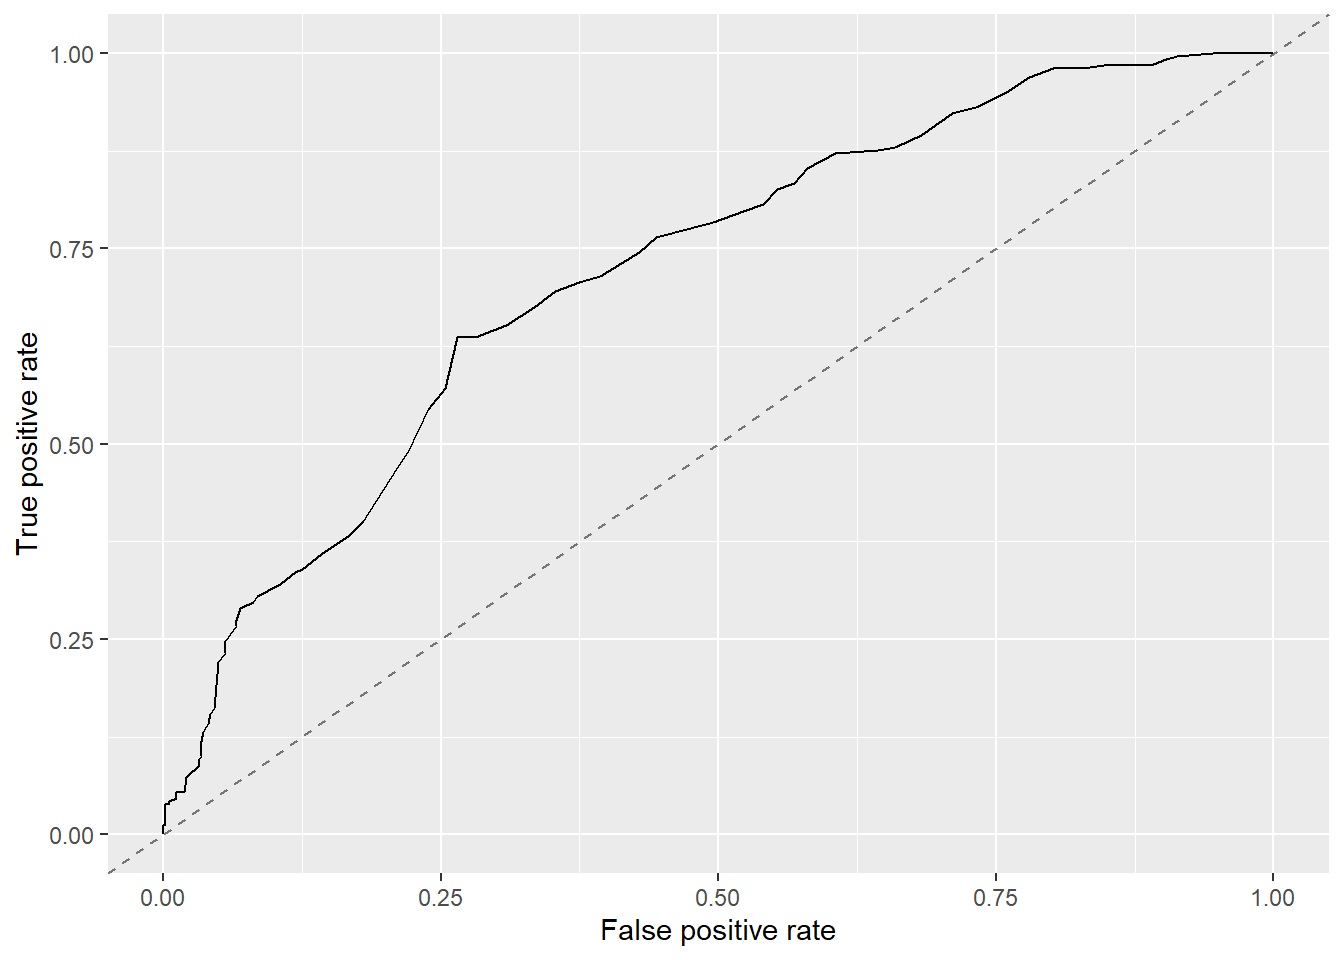
\includegraphics{Variable_Selection_files/figure-latex/roc-plot-1.pdf}

Based on this plot, a FP of around 0.5 an TP of around 0.75 seem to
produce a good model. Digging into the \texttt{df} object, you can find
the raw data underlying the curve in \texttt{df\$data} and will find

\begin{Shaded}
\begin{Highlighting}[]
\KeywordTok{print}\NormalTok{(df}\OperatorTok{$}\NormalTok{data[}\DecValTok{29}\OperatorTok{:}\DecValTok{31}\NormalTok{,])}
\end{Highlighting}
\end{Shaded}

\begin{verbatim}
##          fpr       tpr threshold
## 29 0.4288136 0.7451737 0.2828283
## 30 0.3932203 0.7142857 0.2929293
## 31 0.3745763 0.7065637 0.3030303
\end{verbatim}

This means for this model, if we were to use it we might want to set a
threshold of around 0.3, i.e.~everything above that probability would be
predicted as positive/yes.

\hypertarget{trying-a-different-model}{%
\section{Trying a different model}\label{trying-a-different-model}}

Let's see if we can find another model that might perform even better.
Let's look at a Linear Discriminant Analysis (LDA) model. See
e.g.~chapter 4 of ISLR for more on that model. We again consider AUC as
our measure. The null-model performance is the same, we need to re-do
the remainder.

Let's re-run the single model, followed by the full model and subset
selection.

\begin{Shaded}
\begin{Highlighting}[]
\CommentTok{#copy and paste the code from above for single predictor fits. Switch the learner from a the logistic model to a LDA model. Check the mlr website to figure out the name for that learner. (see 'integrated learner' section)}
\KeywordTok{set.seed}\NormalTok{(}\DecValTok{1111}\NormalTok{) }\CommentTok{#makes each code block reproducible}
\CommentTok{#set learner/model. this corresponds to a logistic model.}
\CommentTok{#mlr calls different models different "learners"}
\NormalTok{learner_name =}\StringTok{ "classif.lda"}\NormalTok{;}
\NormalTok{mylearner =}\StringTok{ }\KeywordTok{makeLearner}\NormalTok{(learner_name, }\DataTypeTok{predict.type =} \StringTok{"prob"}\NormalTok{)}
\CommentTok{# this will contain the results}
\NormalTok{unifmat=}\KeywordTok{data.frame}\NormalTok{(}\DataTypeTok{variable =} \KeywordTok{rep}\NormalTok{(}\DecValTok{0}\NormalTok{,npred), }\DataTypeTok{Accuracy =} \KeywordTok{rep}\NormalTok{(}\DecValTok{0}\NormalTok{,npred))}
\CommentTok{# loop over each predictor, build simple dataset with just outcome and that predictor, fit it to a glm/logistic model}
\ControlFlowTok{for}\NormalTok{ (nn }\ControlFlowTok{in} \DecValTok{1}\OperatorTok{:}\NormalTok{npred)}
\NormalTok{\{}
\NormalTok{    unidata =}\StringTok{ }\KeywordTok{data.frame}\NormalTok{(}\DataTypeTok{gg2c4 =}\NormalTok{ outcome, Outcomefirst[,nn}\OperatorTok{+}\DecValTok{1}\NormalTok{] )}
    \CommentTok{## Generate the task, i.e. define outcome and predictors to be fit}
\NormalTok{    mytask =}\StringTok{ }\KeywordTok{makeClassifTask}\NormalTok{(}\DataTypeTok{id=}\StringTok{'unianalysis'}\NormalTok{, }\DataTypeTok{data =}\NormalTok{ unidata, }\DataTypeTok{target =}\NormalTok{ outcomename, }\DataTypeTok{positive =} \StringTok{"Yes"}\NormalTok{)}
\NormalTok{    model =}\StringTok{ }\KeywordTok{resample}\NormalTok{(mylearner, }\DataTypeTok{task =}\NormalTok{ mytask, }\DataTypeTok{resampling =}\NormalTok{ sampling_choice, }\DataTypeTok{show.info =} \OtherTok{FALSE}\NormalTok{, }\DataTypeTok{measures =}\NormalTok{ mlr }\OperatorTok{::}\StringTok{ }\NormalTok{auc )}
\NormalTok{    unifmat[nn,}\DecValTok{1}\NormalTok{] =}\StringTok{ }\KeywordTok{names}\NormalTok{(predictors)[nn] }
\NormalTok{    unifmat[nn,}\DecValTok{2}\NormalTok{] =}\StringTok{ }\NormalTok{model}\OperatorTok{$}\NormalTok{aggr}
\NormalTok{\}}
\KeywordTok{kable}\NormalTok{(unifmat)}
\end{Highlighting}
\end{Shaded}

\begin{longtable}[]{@{}lr@{}}
\toprule
variable & Accuracy\tabularnewline
\midrule
\endhead
Action1 & 0.5086751\tabularnewline
CasesAll & 0.4464498\tabularnewline
Country & 0.5807351\tabularnewline
Deaths & 0.5161977\tabularnewline
Hemisphere & 0.5076597\tabularnewline
Hospitalizations & 0.5031918\tabularnewline
MeanD1 & 0.4949457\tabularnewline
MeanI1 & 0.5014621\tabularnewline
MedianD1 & 0.5172409\tabularnewline
MedianI1 & 0.5292838\tabularnewline
OBYear & 0.5979801\tabularnewline
Path1 & 0.5130772\tabularnewline
RiskAll & 0.5705659\tabularnewline
season & 0.5862556\tabularnewline
Trans1 & 0.6045373\tabularnewline
Vomit & 0.5294234\tabularnewline
Setting & 0.5625620\tabularnewline
\bottomrule
\end{longtable}

\begin{Shaded}
\begin{Highlighting}[]
\CommentTok{#copy and paste the code from above for the full model fit, but now for LDA. Since you already switched the learner/model above, no further adjustment should be needed}
\KeywordTok{set.seed}\NormalTok{(}\DecValTok{1111}\NormalTok{) }\CommentTok{#makes each code block reproducible}
\CommentTok{#do full model with Cross-Validation - to get an idea for the amount of over-fitting a full model does}
\NormalTok{mytask =}\StringTok{ }\KeywordTok{makeClassifTask}\NormalTok{(}\DataTypeTok{id=}\StringTok{'fullanalysis'}\NormalTok{, }\DataTypeTok{data =}\NormalTok{ Outcomefirst, }\DataTypeTok{target =}\NormalTok{ outcomename, }\DataTypeTok{positive =} \StringTok{"Yes"}\NormalTok{)}
\end{Highlighting}
\end{Shaded}

\begin{verbatim}
## Warning in makeTask(type = type, data = data, weights = weights, blocking =
## blocking, : Empty factor levels were dropped for columns: Country
\end{verbatim}

\begin{Shaded}
\begin{Highlighting}[]
\NormalTok{fullmodel =}\StringTok{ }\KeywordTok{resample}\NormalTok{(mylearner, }\DataTypeTok{task =}\NormalTok{ mytask, }\DataTypeTok{resampling =}\NormalTok{ sampling_choice, }\DataTypeTok{show.info =} \OtherTok{FALSE}\NormalTok{, }\DataTypeTok{measures =}\NormalTok{ mlr }\OperatorTok{::}\StringTok{ }\NormalTok{auc )}
\NormalTok{AUC_fullmodel =}\StringTok{ }\NormalTok{fullmodel}\OperatorTok{$}\NormalTok{aggr[}\DecValTok{1}\NormalTok{]}
\KeywordTok{print}\NormalTok{(AUC_fullmodel)}
\end{Highlighting}
\end{Shaded}

\begin{verbatim}
## auc.test.mean 
##     0.6737898
\end{verbatim}

\begin{Shaded}
\begin{Highlighting}[]
\CommentTok{#copy and paste the code from above for subset selection, now for LDA. Since you already switched the learner/model above, no further adjustment should be needed}
\KeywordTok{set.seed}\NormalTok{(}\DecValTok{1111}\NormalTok{) }
\NormalTok{tstart=}\KeywordTok{proc.time}\NormalTok{(); }\CommentTok{#capture current CPU time for timing how long things take}
\CommentTok{#do 2 forms of forward and backward selection, just to compare}
\NormalTok{select_methods=}\KeywordTok{c}\NormalTok{(}\StringTok{"sbs"}\NormalTok{,}\StringTok{"sfbs"}\NormalTok{,}\StringTok{"sfs"}\NormalTok{,}\StringTok{"sffs"}\NormalTok{) }
\NormalTok{resmat=}\KeywordTok{data.frame}\NormalTok{(}\DataTypeTok{method =} \KeywordTok{rep}\NormalTok{(}\DecValTok{0}\NormalTok{,}\DecValTok{4}\NormalTok{), }\DataTypeTok{Accuracy =} \KeywordTok{rep}\NormalTok{(}\DecValTok{0}\NormalTok{,}\DecValTok{4}\NormalTok{), }\DataTypeTok{Model =} \KeywordTok{rep}\NormalTok{(}\DecValTok{0}\NormalTok{,}\DecValTok{4}\NormalTok{))}
\NormalTok{ct=}\DecValTok{1}\NormalTok{;}
\ControlFlowTok{for}\NormalTok{ (select_method }\ControlFlowTok{in}\NormalTok{ select_methods) }\CommentTok{#loop over all stepwise selection methods}
\NormalTok{\{}
\NormalTok{  ctrl =}\StringTok{ }\KeywordTok{makeFeatSelControlSequential}\NormalTok{(}\DataTypeTok{method =}\NormalTok{ select_method)}
  \KeywordTok{print}\NormalTok{(}\KeywordTok{sprintf}\NormalTok{(}\StringTok{'doing subset selection with method %s '}\NormalTok{,select_method))}
\NormalTok{  sfeat_res =}\StringTok{ }\KeywordTok{selectFeatures}\NormalTok{(}\DataTypeTok{learner =}\NormalTok{ mylearner, }
                             \DataTypeTok{task =}\NormalTok{ mytask, }
                             \DataTypeTok{resampling =}\NormalTok{ sampling_choice, }
                             \DataTypeTok{control =}\NormalTok{ ctrl, }
                             \DataTypeTok{show.info =} \OtherTok{FALSE}\NormalTok{,}
                             \DataTypeTok{measures =}\NormalTok{ mlr }\OperatorTok{::}\StringTok{ }\NormalTok{auc)}
  
\NormalTok{  resmat[ct,}\DecValTok{1}\NormalTok{] =}\StringTok{ }\NormalTok{select_methods[ct]}
\NormalTok{  resmat[ct,}\DecValTok{2}\NormalTok{] =}\StringTok{ }\NormalTok{sfeat_res}\OperatorTok{$}\NormalTok{y}
\NormalTok{  resmat[ct,}\DecValTok{3}\NormalTok{] =}\StringTok{ }\KeywordTok{paste}\NormalTok{(}\KeywordTok{as.vector}\NormalTok{(sfeat_res}\OperatorTok{$}\NormalTok{x), }\DataTypeTok{collapse=} \StringTok{', '}\NormalTok{)}
\NormalTok{  ct=ct}\OperatorTok{+}\DecValTok{1}\NormalTok{;}
\NormalTok{\}}
\end{Highlighting}
\end{Shaded}

\begin{verbatim}
## [1] "doing subset selection with method sbs "
## [1] "doing subset selection with method sfbs "
## [1] "doing subset selection with method sfs "
## [1] "doing subset selection with method sffs "
\end{verbatim}

\begin{Shaded}
\begin{Highlighting}[]
\CommentTok{# do feature selection with genetic algorithm}
\NormalTok{maxit =}\StringTok{ }\DecValTok{100} \CommentTok{#number of iterations - should be large for 'production run'}
\NormalTok{ctrl_GA =}\KeywordTok{makeFeatSelControlGA}\NormalTok{(}\DataTypeTok{maxit =}\NormalTok{ maxit)}
\KeywordTok{print}\NormalTok{(}\KeywordTok{sprintf}\NormalTok{(}\StringTok{'doing subset selection with genetic algorithm'}\NormalTok{))}
\end{Highlighting}
\end{Shaded}

\begin{verbatim}
## [1] "doing subset selection with genetic algorithm"
\end{verbatim}

\begin{Shaded}
\begin{Highlighting}[]
\NormalTok{sfeatga_res =}\StringTok{ }\KeywordTok{selectFeatures}\NormalTok{(}\DataTypeTok{learner =}\NormalTok{ mylearner, }
                                   \DataTypeTok{task =}\NormalTok{ mytask, }
                                   \DataTypeTok{resampling =}\NormalTok{ sampling_choice, }
                                   \DataTypeTok{control =}\NormalTok{ ctrl_GA, }
                                   \DataTypeTok{show.info =} \OtherTok{FALSE}\NormalTok{,}
                                   \DataTypeTok{measures =}\NormalTok{ mlr }\OperatorTok{::}\StringTok{ }\NormalTok{auc)}
\NormalTok{resmat[}\DecValTok{5}\NormalTok{,}\DecValTok{1}\NormalTok{] =}\StringTok{ "GA"}
\NormalTok{resmat[}\DecValTok{5}\NormalTok{,}\DecValTok{2}\NormalTok{] =}\StringTok{ }\NormalTok{sfeatga_res}\OperatorTok{$}\NormalTok{y}
\NormalTok{resmat[}\DecValTok{5}\NormalTok{,}\DecValTok{3}\NormalTok{] =}\StringTok{ }\KeywordTok{paste}\NormalTok{(}\KeywordTok{as.vector}\NormalTok{(sfeatga_res}\OperatorTok{$}\NormalTok{x), }\DataTypeTok{collapse=} \StringTok{', '}\NormalTok{)}
\NormalTok{runtime.minutes_SS=(}\KeywordTok{proc.time}\NormalTok{()}\OperatorTok{-}\NormalTok{tstart)[[}\DecValTok{3}\NormalTok{]]}\OperatorTok{/}\DecValTok{60}\NormalTok{; }\CommentTok{#total time in minutes the optimization took}
\KeywordTok{print}\NormalTok{(}\KeywordTok{sprintf}\NormalTok{(}\StringTok{'subset selection took %f minutes'}\NormalTok{,runtime.minutes_SS));}
\end{Highlighting}
\end{Shaded}

\begin{verbatim}
## [1] "subset selection took 2.891167 minutes"
\end{verbatim}

\begin{Shaded}
\begin{Highlighting}[]
\KeywordTok{kable}\NormalTok{(resmat)}
\end{Highlighting}
\end{Shaded}

\begin{longtable}[]{@{}lrl@{}}
\toprule
method & Accuracy & Model\tabularnewline
\midrule
\endhead
sbs & 0.6875153 & Action1, Country, Deaths, MedianI1, OBYear, RiskAll,
season, Trans1, Setting\tabularnewline
sfbs & 0.6862458 & Action1, Country, Deaths, MedianI1, OBYear, RiskAll,
season, Trans1, Setting\tabularnewline
sfs & 0.6625805 & Country, OBYear, season, Trans1\tabularnewline
sffs & 0.6714397 & Country, OBYear, season, Trans1,
Setting\tabularnewline
GA & 0.6846441 & Action1, Country, Deaths, MedianI1, OBYear, RiskAll,
season, Trans1, Setting\tabularnewline
\bottomrule
\end{longtable}

It Looks like we again get some sub-models that are slightly better than
the full model, at least as evaluated using the (cross-validated) AUC
measure. There seems to be a bit, but not much difference in performance
to the logistic model. We can take the GA model again (because it's
conveniently at the end, even if it's not the best) and look at its ROC
and compare the curves for the LDA and logistic models.

\begin{Shaded}
\begin{Highlighting}[]
\CommentTok{#copy the code from roc-plot above and re-do train/predict byt now save it as lda_mod and lda_pred}
\CommentTok{#then use generateThreshVsPerfData() with both lda_pred and log_pred (computed above) to create a structure that contains}
\CommentTok{#best model curves for both logistic and LDA, then plot the curves.}
\KeywordTok{set.seed}\NormalTok{(}\DecValTok{1111}\NormalTok{) }\CommentTok{#makes each code block reproducible}
\NormalTok{d2 <-}\StringTok{ }\NormalTok{Outcomefirst }\OperatorTok\StringTok{ }\NormalTok{dplyr}\OperatorTok{::}\KeywordTok{select}\NormalTok{(gg2c4, sfeatga_res}\OperatorTok{$}\NormalTok{x )}
\NormalTok{mytask =}\StringTok{ }\KeywordTok{makeClassifTask}\NormalTok{(}\DataTypeTok{id=}\StringTok{'rocanalysis'}\NormalTok{, }\DataTypeTok{data =}\NormalTok{ d2, }\DataTypeTok{target =}\NormalTok{ outcomename, }\DataTypeTok{positive =} \StringTok{"Yes"}\NormalTok{)}
\end{Highlighting}
\end{Shaded}

\begin{verbatim}
## Warning in makeTask(type = type, data = data, weights = weights, blocking =
## blocking, : Empty factor levels were dropped for columns: Country
\end{verbatim}

\begin{Shaded}
\begin{Highlighting}[]
\NormalTok{lda_mod =}\StringTok{ }\KeywordTok{train}\NormalTok{(mylearner, mytask)}
\NormalTok{lda_pred =}\StringTok{ }\KeywordTok{predict}\NormalTok{(lda_mod, }\DataTypeTok{task =}\NormalTok{ mytask)}
\NormalTok{df =}\StringTok{ }\KeywordTok{generateThreshVsPerfData}\NormalTok{(}\KeywordTok{list}\NormalTok{(}\DataTypeTok{LDA =}\NormalTok{ lda_pred, }\DataTypeTok{logistic =}\NormalTok{ log_pred), }\DataTypeTok{measures =} \KeywordTok{list}\NormalTok{(fpr, tpr))}
\KeywordTok{plotROCCurves}\NormalTok{(df)}
\end{Highlighting}
\end{Shaded}

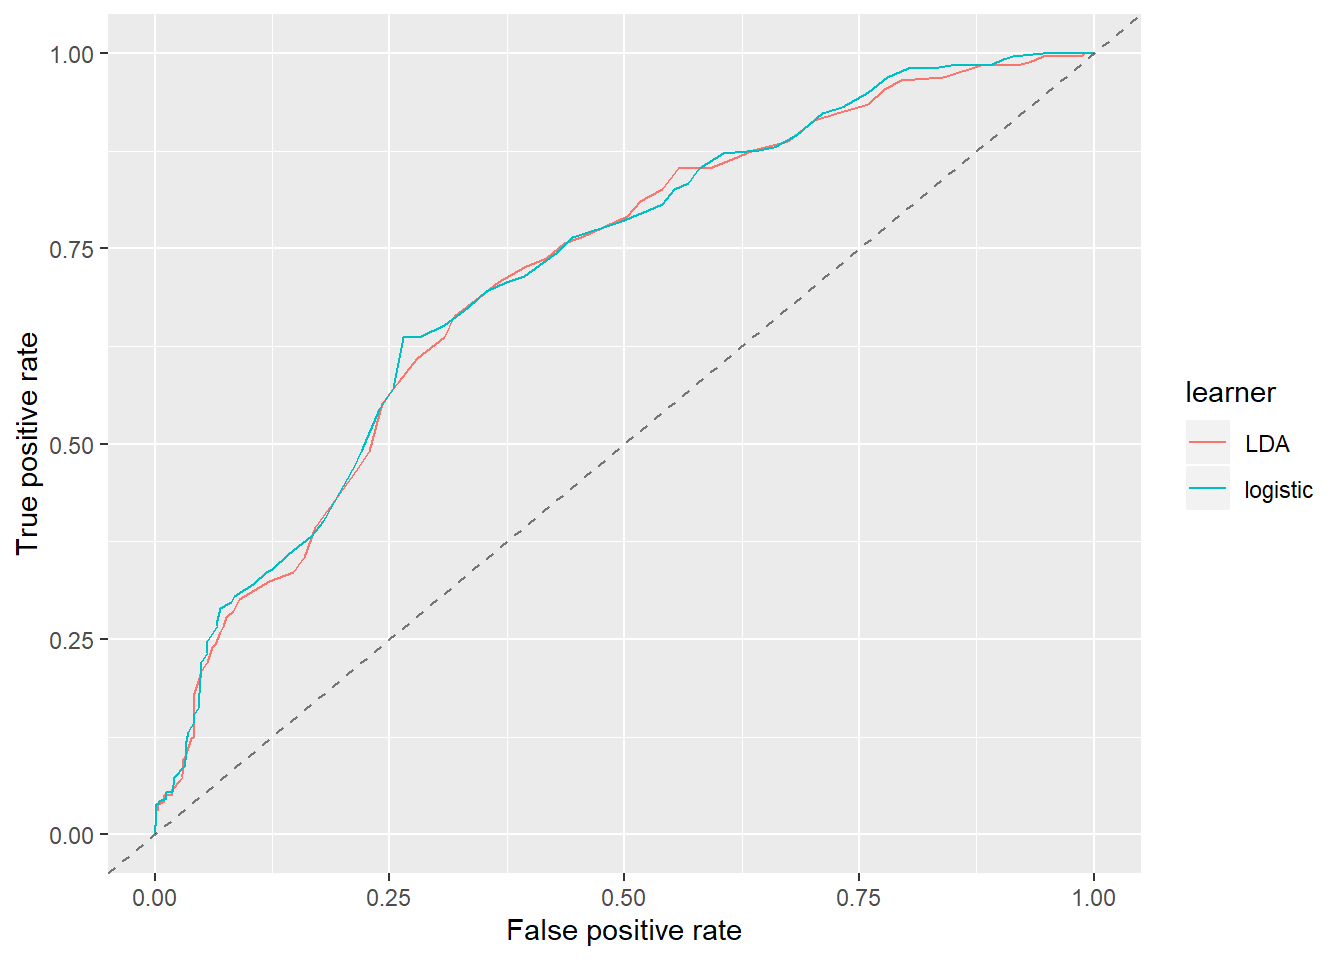
\includegraphics{Variable_Selection_files/figure-latex/roc-plot-2-1.pdf}

You should see from the plot that the LDA model performs very similar to
the Logistic model.

\begin{Shaded}
\begin{Highlighting}[]
\CommentTok{#close down the parallelization started at the beginning to free up resources.}
\KeywordTok{parallelStop}\NormalTok{()}
\end{Highlighting}
\end{Shaded}

\hypertarget{wrapping-up}{%
\section{Wrapping up}\label{wrapping-up}}

Based on the above, we could choose a model simply by best performance.
However, we likely also still want to look at model prediction
uncertainty and do some residual plots and other diagnostics for our
chosen model before we finalize our choice. As was the case for
\texttt{caret}, \texttt{mlr} also comes with lots of functions that make
these - and many other - tasks easier. We'll leave it at this for now,
and might revisit some of those topics in further exercises.

Also, none of the models here are that great. We might want to think
more about our initial premise, i.e.~looking for associations between
virus strain type and other variables and what the scientific rationale
is for expecting variations. Here, we just ran the model and looked what
we might find. That approach, sometimes called \emph{data exploration}
or \emph{data mining} or - less charitable \emph{fishing expedition} is
ok, but we need to be careful how we interpret and use the results.
Going in with a clear hypothesis is usually better.

\hypertarget{a-few-more-comments}{%
\section{A few more comments}\label{a-few-more-comments}}

Things are getting a bit slow now, despite the multiple cores we need
minutes to run things. Also, code chunks get larger. At this point, it
might be worth considering a structure whereby most of the code lives in
one or several \textbf{well documented} R scripts, which can be run
independently. Those R scripts should save their results, and those
results are then loaded here. The advantage is that if one wants to make
changes to a small part of the analysis, one can modify and run just
that part and update the whole document by re-knitting without having to
run all code. For any big/serious analysis, I suggest such a setup that
splits R code from RMarkdown files, at least for the computationally
intensive parts.


\end{document}
